% SPDX-License-Identifier: MIT
% The MakeYourTree user manual.
% Build with:  python docs/manual/build.py
%
% Figures are the vector PDFs in examples/gallery/, written by
% tools/make_gallery.py. Run that first if the build reports them missing.

\documentclass[11pt,a4paper,openany]{book}

% ---------------------------------------------------------------- page setup
\usepackage[a4paper,top=27mm,bottom=27mm,inner=28mm,outer=24mm]{geometry}
\usepackage[T1]{fontenc}
\usepackage[utf8]{inputenc}
\usepackage{lmodern}
\usepackage{microtype}
\usepackage{graphicx}
\usepackage{xcolor}
\usepackage{booktabs}
\usepackage{longtable}
\usepackage{array}
\usepackage{enumitem}
\usepackage{titlesec}
\usepackage{fancyhdr}
\usepackage{listings}
\usepackage{caption}
\usepackage{tikz}

\graphicspath{{../../examples/gallery/}}

% ------------------------------------------------------------------- colours
\definecolor{mytBlue}{HTML}{2166AC}
\definecolor{mytInk}{HTML}{1A1A22}
\definecolor{mytGrey}{HTML}{5A5A66}
\definecolor{mytRule}{HTML}{C8C8D0}
\definecolor{mytWash}{HTML}{F2F4F7}
\definecolor{mytGreen}{HTML}{117733}
\definecolor{mytRed}{HTML}{B2182B}

% ------------------------------------------------------------------ hyperref
% Loaded late, as it patches a great deal. bookmark then fixes the nesting of
% the PDF outline, which is what makes the sidebar navigation behave.
\usepackage[
  colorlinks=true,
  linkcolor=mytBlue,
  urlcolor=mytBlue,
  citecolor=mytBlue,
  bookmarksnumbered=true,
  bookmarksopen=true,
  bookmarksopenlevel=1,
  pdftitle={MakeYourTree User Manual},
  pdfauthor={Manish Prakash Victor},
  pdfsubject={Phylogenetic tree visualisation and annotation},
  pdfkeywords={phylogenetics, tree visualisation, Newick, NEXUS, phyloXML},
  pdfdisplaydoctitle=true
]{hyperref}
\usepackage{bookmark}

% --------------------------------------------------------------- heading style
\titleformat{\chapter}[display]
  {\normalfont\sffamily\huge\bfseries\color{mytInk}}
  {\normalsize\sffamily\bfseries\color{mytBlue}\MakeUppercase{\chaptertitlename}\ \thechapter}
  {12pt}{\Huge}
\titleformat{\section}
  {\normalfont\sffamily\Large\bfseries\color{mytInk}}{\thesection}{1em}{}
\titleformat{\subsection}
  {\normalfont\sffamily\large\bfseries\color{mytInk}}{\thesubsection}{1em}{}

\pagestyle{fancy}
\fancyhf{}
\renewcommand{\headrulewidth}{0.4pt}
\fancyhead[L]{\small\sffamily\color{mytGrey}\nouppercase{\leftmark}}
\fancyhead[R]{\small\sffamily\color{mytGrey}\thepage}
\fancypagestyle{plain}{\fancyhf{}\renewcommand{\headrulewidth}{0pt}%
  \fancyfoot[C]{\small\sffamily\color{mytGrey}\thepage}}

\captionsetup{font=small,labelfont={sf,bf},textfont=sf,labelsep=period}

% ------------------------------------------------------------------- listings
\lstdefinestyle{myt}{
  basicstyle=\ttfamily\small\color{mytInk},
  backgroundcolor=\color{mytWash},
  frame=single,
  rulecolor=\color{mytRule},
  framesep=6pt,
  xleftmargin=10pt,
  xrightmargin=4pt,
  breaklines=true,
  breakatwhitespace=true,
  showstringspaces=false,
  keywordstyle=\color{mytBlue}\bfseries,
  commentstyle=\color{mytGreen}\itshape,
  stringstyle=\color{mytRed},
  columns=fullflexible,
}
\lstset{style=myt}
\lstdefinelanguage{mytrack}{
  morekeywords={type,title,match,thickness,colors,legend,names,show},
  morecomment=[l]{\#},
  sensitive=false,
}

% ------------------------------------------------------------------- macros
\newcommand{\app}{MakeYourTree}
\newcommand{\studio}{\app{} Studio}
\newcommand{\cmd}[1]{\texttt{#1}}
\newcommand{\opt}[1]{\texttt{#1}}

% A keycap. Boxed rather than merely monospaced, so a shortcut is never mistaken
% for a filename in running text.
\newcommand{\keys}[1]{%
  \tikz[baseline=(K.base)]\node[inner xsep=3.5pt,inner ysep=1.6pt,
    rounded corners=2pt,draw=mytRule,fill=mytWash,line width=0.5pt](K)
    {\footnotesize\sffamily\color{mytInk}#1};}

% A gallery figure with a caption. #1 file stem, #2 caption, #3 width fraction.
\newcommand{\galleryfig}[3]{%
  \begin{figure}[htbp]\centering
    \includegraphics[width=#3\linewidth]{#1}
    \caption{#2}\label{fig:#1}
  \end{figure}}

\setlist{itemsep=2pt,parsep=0pt,topsep=4pt}
\renewcommand{\arraystretch}{1.25}

\begin{document}

% ---------------------------------------------------------------- title page
\begin{titlepage}
\thispagestyle{empty}
\centering
\vspace*{2.2cm}

{\sffamily\bfseries\fontsize{44}{50}\selectfont\color{mytInk} MakeYourTree}

\vspace{6mm}
{\sffamily\Large\color{mytGrey} Phylogenetic tree visualisation and annotation}

\vspace{4mm}
{\color{mytBlue}\rule{0.55\linewidth}{1.2pt}}

\vspace{10mm}
{\sffamily\LARGE\color{mytInk} User Manual}

\vspace{3mm}
{\sffamily\large\color{mytGrey} Version 0.1.0}

\vspace{12mm}
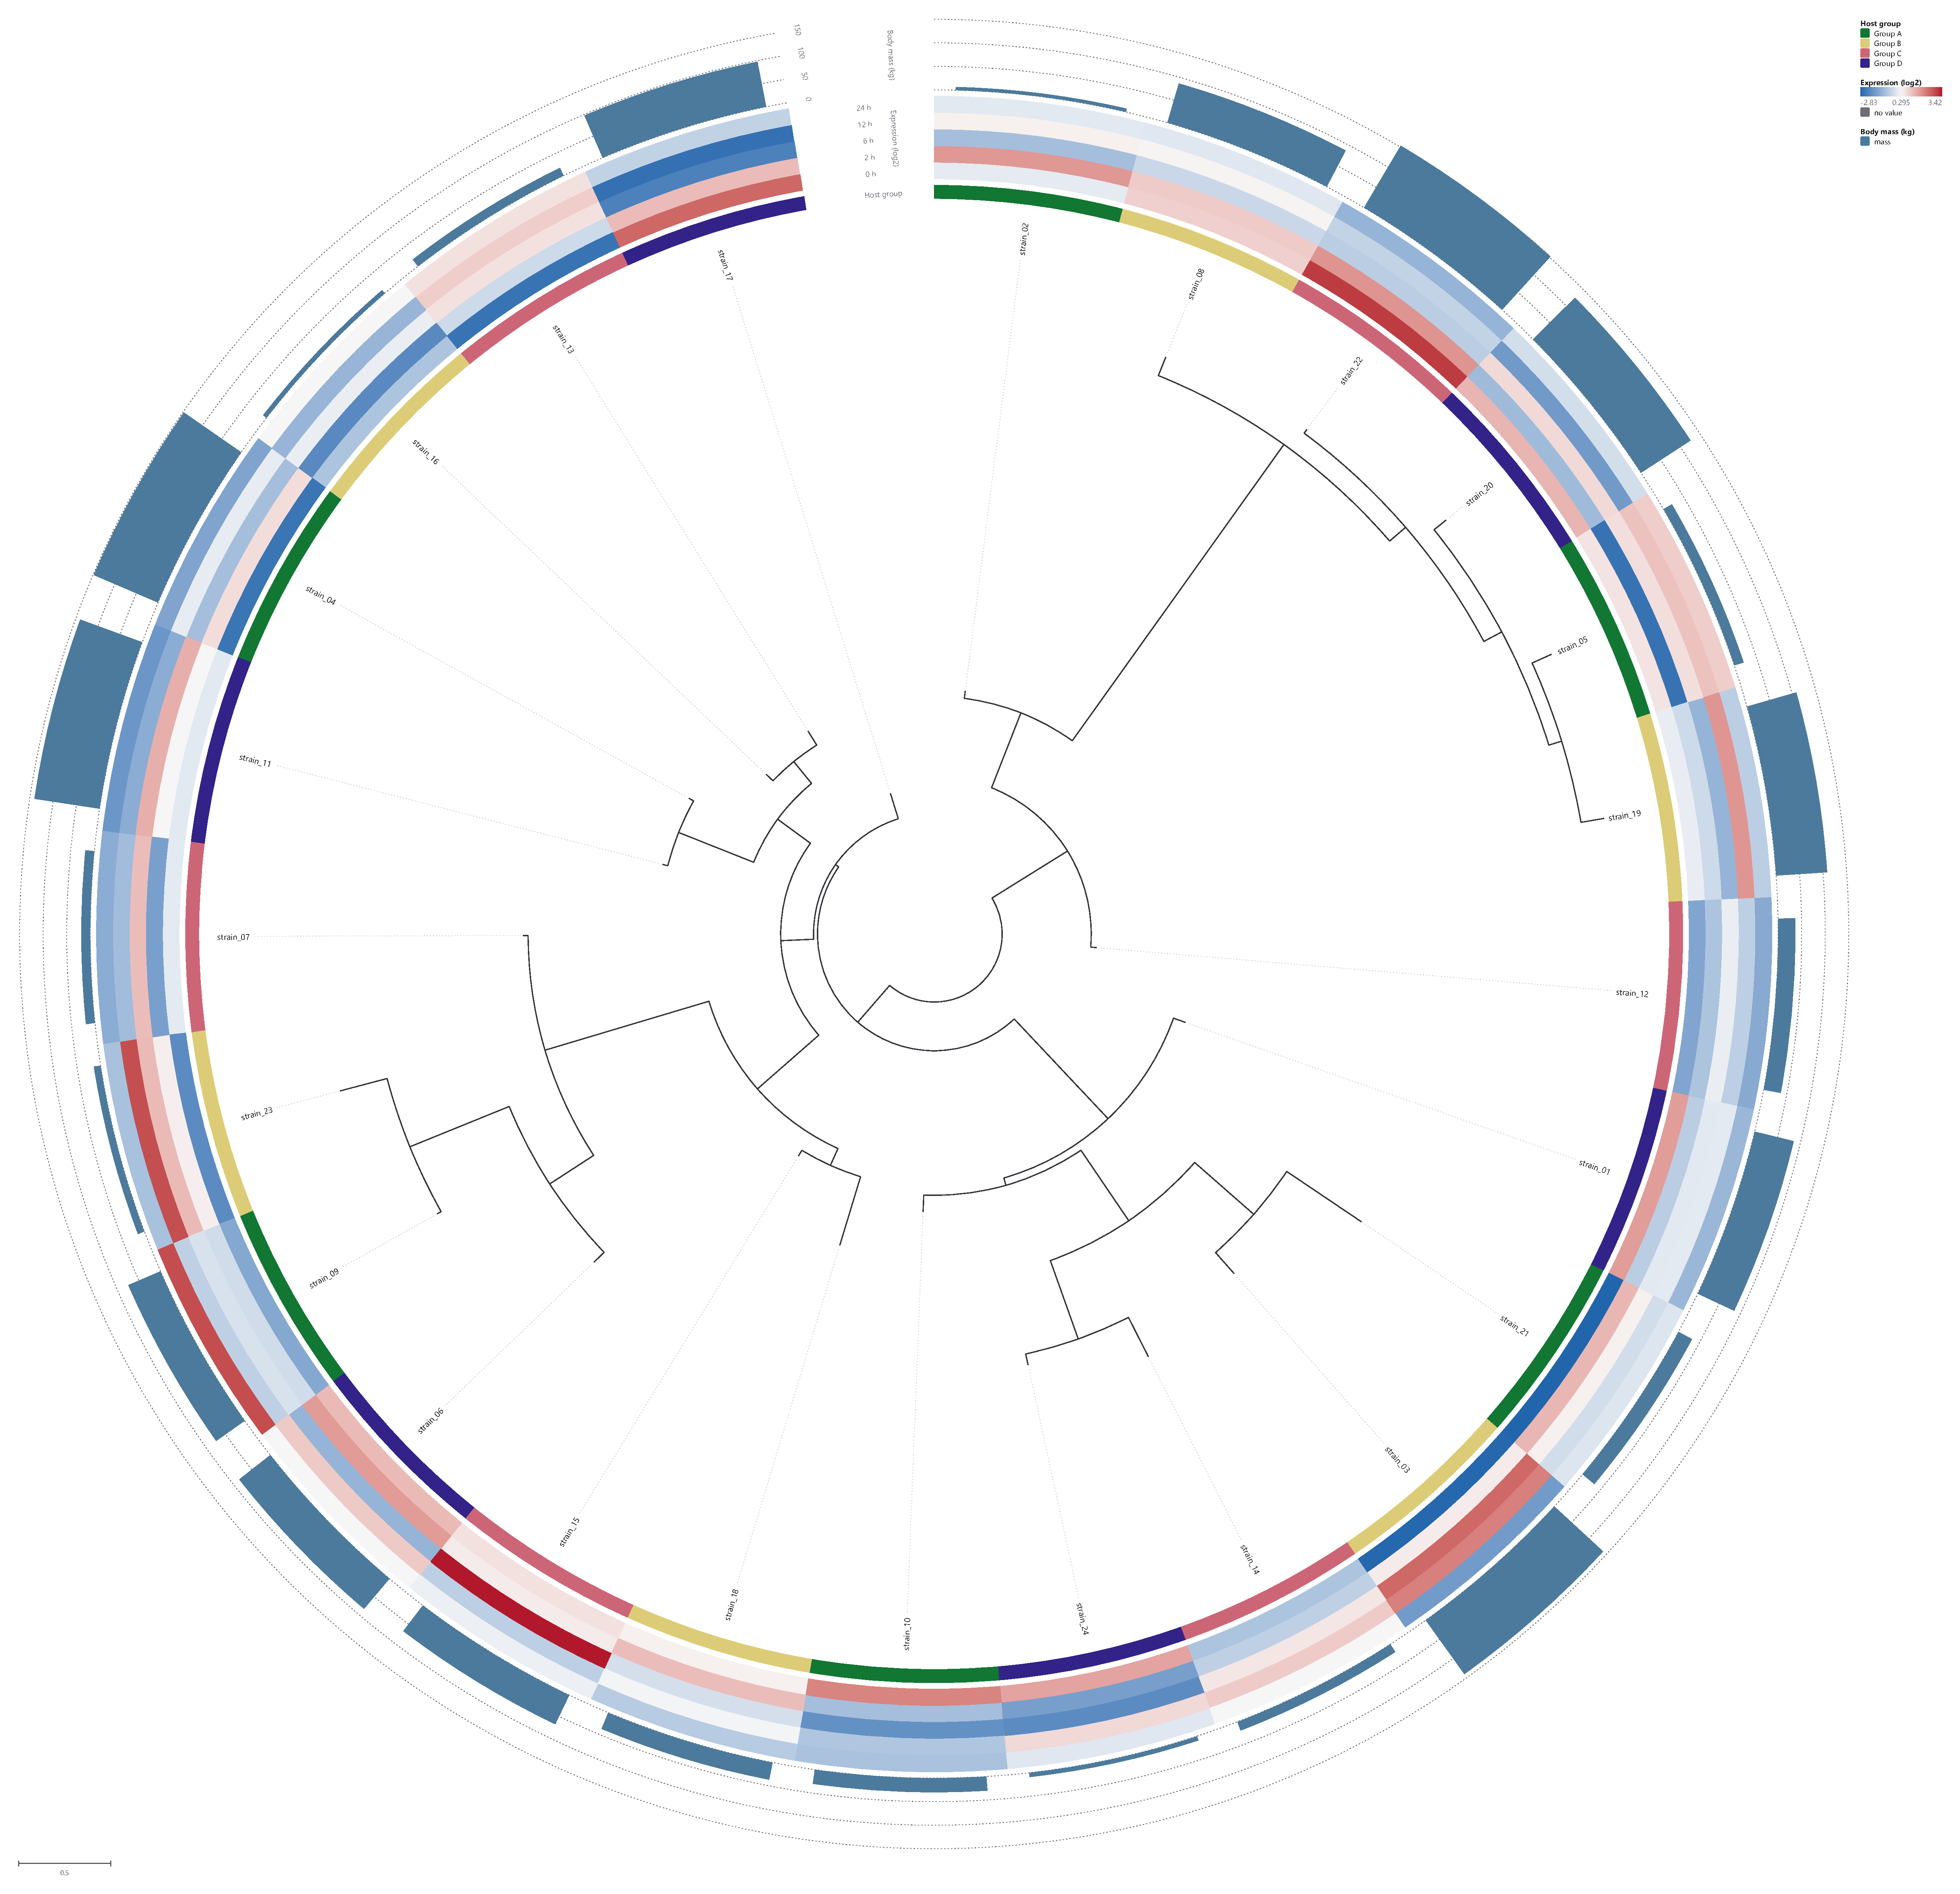
\includegraphics[width=0.86\linewidth]{combined-circular}

\vfill
{\sffamily\color{mytGrey}
Manish Prakash Victor\\[2mm]
Free and open-source software under the MIT licence\\
No server. No account. No network access at runtime.}

\vspace{8mm}
\end{titlepage}

% ------------------------------------------------------------ colophon page
\thispagestyle{empty}
\noindent\textbf{\sffamily \app{} User Manual}\\
Version 0.1.0, for \app{} 0.1.0.

\vspace{4mm}
\noindent Copyright \copyright{} 2026 Manish Prakash Victor.

\vspace{2mm}
\noindent \app{} is free and open-source software, released under the MIT licence.
You may use, copy, modify and redistribute it, including commercially. The
software is provided without warranty of any kind. The full text is in
\cmd{LICENSES/MIT.txt} in the source repository.

\vspace{2mm}
\noindent This manual is released under the same terms. Every figure in it was
produced by \app{} itself, from the synthetic datasets in \cmd{examples/}, by
running \cmd{python tools/make\_gallery.py}.

\vspace{4mm}
\noindent \app{} is an independent implementation. It is not affiliated with,
endorsed by, or derived from any other phylogenetics package.

\vspace{4mm}
\noindent The desktop application links PySide6/Qt~6, which is distributed under
the LGPL-3.0. If you redistribute a compiled bundle, that licence places
conditions on you; see \cmd{LICENSE.md} in the repository.

\vfill
\noindent{\small\sffamily\color{mytGrey}Typeset with \LaTeX.}

\cleardoublepage

% ---------------------------------------------------------------------- TOC
\pagenumbering{roman}
\setcounter{tocdepth}{1}
\pdfbookmark[0]{Contents}{toc}
\tableofcontents
\cleardoublepage
\pagenumbering{arabic}

% ------------------------------------------------------------------- content
\part{Getting started}
% SPDX-License-Identifier: MIT
\chapter{Introduction}
\label{ch:introduction}

\app{} is a desktop application and Python library for visualising and annotating
phylogenetic trees. It runs entirely on your own machine: there is no server, no
account, no upload and no network access at any point while it runs.

\section{What it does}

\begin{description}[style=nextline,leftmargin=0pt,labelindent=0pt,labelwidth=0pt]
  \item[Reads what you already have.]
    Newick, New Hampshire eXtended (NHX), NEXUS and phyloXML. Parsing is
    deliberately forgiving --- real files break their specifications constantly,
    so \app{} loads them anyway and tells you what it had to interpret.
  \item[Draws it many ways.]
    Rectangular and slanted phylograms and cladograms, circular fans with a
    configurable arc and inner radius, radial layouts, and unrooted layouts by
    Felsenstein's equal-angle and equal-daylight algorithms.
  \item[Lets you edit the tree.]
    Reroot on any branch, by outgroup or at the midpoint; ladderize, rotate,
    collapse, prune and extract subtrees. Everything is undoable.
  \item[Annotates it.]
    Thirteen track types stack alongside the tree, described in
    Chapter~\ref{ch:tracks}.
  \item[Exports honestly.]
    SVG and PDF as vectors, PNG at any resolution. The on-screen canvas and the
    exported file are built from an identical description, so what you export is
    what you saw.
\end{description}

\section{Who it is for}

Anyone who has a tree and needs a figure of it: for a paper, a thesis, a talk or
a teaching handout. It is aimed particularly at people who cannot or would rather
not upload their data to a hosted service --- unpublished phylogenies, clinical
isolate data, or work under a data-transfer agreement. Nothing leaves your
machine, because the software has no way to send it anywhere.

The library half is aimed at a different need: regenerating a figure
reproducibly, from a script, as part of an analysis pipeline. Anything you can
build interactively you can also build in Python (Chapter~\ref{ch:python}) or
from the command line (Chapter~\ref{ch:cli}).

\section{Two packages}

\app{} ships as two Python packages, and the split is architectural rather than
legal --- both are MIT-licensed.

\begin{center}
\begin{tabular}{@{}lp{0.62\linewidth}@{}}
\toprule
\textbf{Package} & \textbf{Contents} \\
\midrule
\cmd{makeyourtree} &
  Parsers, tree model, layout engine, annotation model, scene graph, SVG
  renderer and the command-line interface. Imports no GUI toolkit, so it works
  headlessly in scripts, notebooks and continuous integration. Depends only on
  NumPy. \\
\cmd{makeyourtree\_studio} &
  The desktop application, built on PySide6/Qt~6. \\
\bottomrule
\end{tabular}
\end{center}

If you only want to generate figures from a script, you never need the second
package, and you can install without Qt entirely (Section~\ref{sec:install-library}).

\section{Three ideas behind the design}
\label{sec:design}

You do not need this section to use \app{}. It is here because it explains why
certain things behave the way they do.

\subsection{Two independent coordinates}

Every layout is built from two coordinates that are computed separately. The
\emph{cross} coordinate --- $y$ in a rectangular layout, angle in a circular one
--- comes only from the order of the tips. The \emph{along} coordinate --- $x$,
or radius --- comes only from branch length, or from depth in a cladogram.

The practical consequence is that the two things you do to a figure never
interfere. Ladderizing or rotating a clade changes the ordering and cannot alter
any distance; switching between a phylogram and a cladogram changes the distances
and cannot alter the ordering.

\subsection{Band space: why one track works in every layout}

Annotation tracks are not written for a particular layout. Each is written in
\emph{band space}, a coordinate system of \texttt{(row, offset)} where
\texttt{row} indexes the tip and \texttt{offset} is the distance outward from the
tree. A projector then maps band space into the page: a straight-line mapping for
linear layouts, a polar one for circular layouts.

This is why a heatmap becomes an annulus in a circular layout without you doing
anything, and why tangential labels stay the right way up on the left-hand side
of a fan. Figures~\ref{fig:combined-rectangular} and~\ref{fig:combined-circular}
are the same tracks with the same data; only the layout mode differs.

\subsection{One scene, many outputs}

Laying out and composing a figure produces a plain description of shapes and
text. The on-screen canvas draws that description, and so do the SVG, PDF and PNG
exporters. Because there is only one description, the screen and the file cannot
disagree.

\section{About this manual}

Chapters~\ref{ch:installation}--\ref{ch:quickstart} get you running.
Chapters~\ref{ch:interface}--\ref{ch:editing} cover the application.
Chapters~\ref{ch:annotation}--\ref{ch:tracks} cover annotation, and
Chapter~\ref{ch:tracks} is the reference for all thirteen track types.
Chapters~\ref{ch:export}--\ref{ch:python} cover output and automation.

Every figure in this manual was produced by \app{} from the synthetic example
data in the repository. Nothing is a mock-up.

% SPDX-License-Identifier: MIT
\chapter{Installation}
\label{ch:installation}

\app{} runs on Windows, macOS and Linux from a single environment definition. The
commands are the same on all three; the environment resolves the platform
differences, including the Qt system libraries that would otherwise have to be
installed by hand on Linux.

\app{} is not on PyPI, so installation is from the source repository. There is no
\cmd{pip install makeyourtree} from the index --- ignore any package by that name
from another author.

\section{Requirements}

\begin{itemize}
  \item \cmd{git}
  \item A conda-family package manager, or Python 3.12 or newer for the pip route
  \item About 1\,GB of disk space. Most of that is Qt: a complete environment
        measures 751\,MB, of which PySide6 is 641\,MB and NumPy 34\,MB.
\end{itemize}

No network access is needed at runtime --- only to install.

\section{With conda or mamba}

This is the recommended route. Substitute \cmd{mamba} or \cmd{micromamba} for
\cmd{conda} throughout if you prefer; the arguments are identical and mamba
resolves considerably faster.

\begin{lstlisting}[language=bash]
git clone https://github.com/bioforkgithub/makeyourtree.git
cd makeyourtree
conda env create -f environment.yml
conda activate makeyourtree
pip install -e . --no-deps
\end{lstlisting}

\begin{quote}
\textbf{\opt{--no-deps} is not optional bookkeeping.} Conda has already installed
everything \app{} needs. A plain \cmd{pip install -e .} would resolve those same
requirements again from PyPI and install a \emph{second} copy of Qt into an
environment that already has one --- 641\,MB wasted, and two Qt builds present
where which one loads depends on import order.
\end{quote}

\href{https://github.com/conda-forge/miniforge}{Miniforge} is the usual
recommendation for the package manager itself: it is small and defaults to the
conda-forge channel, which is where \cmd{pyside6} comes from. On Anaconda or
Miniconda the \cmd{defaults} channel takes priority and does not carry
\cmd{pyside6}; if the environment fails to solve, prefer conda-forge:

\begin{lstlisting}[language=bash]
conda config --add channels conda-forge
conda config --set channel_priority strict
\end{lstlisting}

\section{With pip and venv}

Use this if you would rather not install conda. It needs Python 3.12 or newer
already present, and on Linux it needs the Qt system libraries installed by hand
(Section~\ref{sec:linux-libs}).

\begin{lstlisting}[language=bash]
git clone https://github.com/bioforkgithub/makeyourtree.git
cd makeyourtree
python -m venv .venv
\end{lstlisting}

Activate it. This is the only command in this manual that differs by platform:

\begin{center}
\begin{tabular}{@{}ll@{}}
\toprule
\textbf{Platform} & \textbf{Command} \\
\midrule
Linux, macOS         & \cmd{source .venv/bin/activate} \\
Windows, PowerShell  & \cmd{.venv\textbackslash Scripts\textbackslash Activate.ps1} \\
Windows, \cmd{cmd.exe} & \cmd{.venv\textbackslash Scripts\textbackslash activate.bat} \\
\bottomrule
\end{tabular}
\end{center}

Then install. Note that here pip \emph{does} resolve dependencies, so there is no
\opt{--no-deps}:

\begin{lstlisting}[language=bash]
pip install -e ".[studio]"
\end{lstlisting}

\section{The library alone, without Qt}
\label{sec:install-library}

The \cmd{makeyourtree} package and its command-line interface import no GUI
toolkit, so they install without Qt. This is the right choice for a server, a
container, a CI job or an analysis pipeline: it avoids the 641\,MB PySide6 brings
and needs none of the Linux system libraries below.

\begin{lstlisting}[language=bash]
pip install -e "."
\end{lstlisting}

You then have the \cmd{makeyourtree} command and the Python API, but not
\cmd{makeyourtree-studio}. NumPy is the only dependency. With conda, delete the
\cmd{pyside6} line from \cmd{environment.yml} before creating the environment.

\section{Checking the installation}

\begin{lstlisting}[language=bash]
makeyourtree --version
makeyourtree info examples/primates.nwk
\end{lstlisting}

To run the test suite as well --- the fastest way to confirm a healthy install:

\begin{lstlisting}[language=bash]
pip install -e ".[studio,dev]"
python -m pytest
\end{lstlisting}

Expect \textbf{2074 passed} in roughly 30 seconds. The suite runs headlessly and
needs no display.

\section{Platform notes}

Two things genuinely differ by operating system. Both affect the pip route only;
the conda environment handles the first and largely avoids the second.

\subsection{Linux: Qt system libraries}
\label{sec:linux-libs}

The PySide6 \emph{wheel} bundles Qt itself, but Qt still loads a few system
libraries --- above all its \cmd{xcb} platform plugin. Without them the
application exits with
\cmd{qt.qpa.plugin: Could not load the Qt platform plugin "xcb"}.

\begin{lstlisting}[language=bash]
# Debian / Ubuntu
sudo apt install libgl1 libegl1 libglib2.0-0 libfontconfig1 libdbus-1-3 \
  libxkbcommon-x11-0 libxcb-cursor0 libxcb-icccm4 libxcb-image0 \
  libxcb-keysyms1 libxcb-randr0 libxcb-render-util0 libxcb-shape0 \
  libxcb-xinerama0

# Fedora
sudo dnf install mesa-libGL mesa-libEGL fontconfig dbus-libs \
  libxkbcommon-x11 xcb-util-cursor xcb-util-image xcb-util-keysyms \
  xcb-util-renderutil xcb-util-wm
\end{lstlisting}

\cmd{libxcb-cursor0} is required by Qt~6.5 and later specifically, and is the one
most often missing on otherwise complete systems. On Debian and Ubuntu,
\cmd{python3.12-venv} is also a separate package.

\subsection{Windows: clone to a short path}

PySide6 ships files whose names exceed Windows' 260-character \cmd{MAX\_PATH}
limit. Installing into a \cmd{.venv} inside a deeply nested directory fails with
\cmd{OSError: [WinError 206] The filename or extension is too long}, and it rolls
back \emph{partially} --- which is confusing, because the test suite still passes
while \cmd{makeyourtree} itself is missing.

Clone somewhere short such as \cmd{C:\textbackslash dev\textbackslash makeyourtree},
or enable long paths with \cmd{git config -{}-system core.longpaths true} together
with the \cmd{LongPathsEnabled} registry setting. The conda route mostly sidesteps
this, because the environment lives under the conda installation rather than
inside the clone.

\section{Building a standalone bundle}

To produce a self-contained directory that runs without Python installed:

\begin{lstlisting}[language=bash]
pip install pyinstaller
python -m makeyourtree_studio.packaging.build
\end{lstlisting}

The result is \cmd{dist/MakeYourTreeStudio/}. The build driver verifies the
bundle against thirteen checks --- licence texts present, Qt shipped as separate
replaceable shared libraries, no GPL-3.0-only Qt add-on pulled in --- and refuses
to certify one that fails.

PyInstaller cannot cross-build: each platform's bundle must be produced on that
platform. At the time of writing this has been built and launched on Windows
only; macOS and Linux bundles are unproven rather than broken.

% SPDX-License-Identifier: MIT
\chapter{Quick start}
\label{ch:quickstart}

This chapter produces a finished, annotated figure in about five minutes. It uses
the example data in the repository, so you can follow it exactly before
substituting your own tree.

\section{Your first figure, from the command line}

The fastest route to a figure needs no interface at all:

\begin{lstlisting}[language=bash]
makeyourtree render examples/primates.nwk figure.svg
\end{lstlisting}

That writes a rectangular phylogram as a vector SVG. Add a layout and an
annotation track:

\begin{lstlisting}[language=bash]
makeyourtree render examples/primates.nwk figure.svg \
    --mode circular --align-tips \
    --track examples/primates_region.mytrack
\end{lstlisting}

\begin{figure}[htbp]\centering
  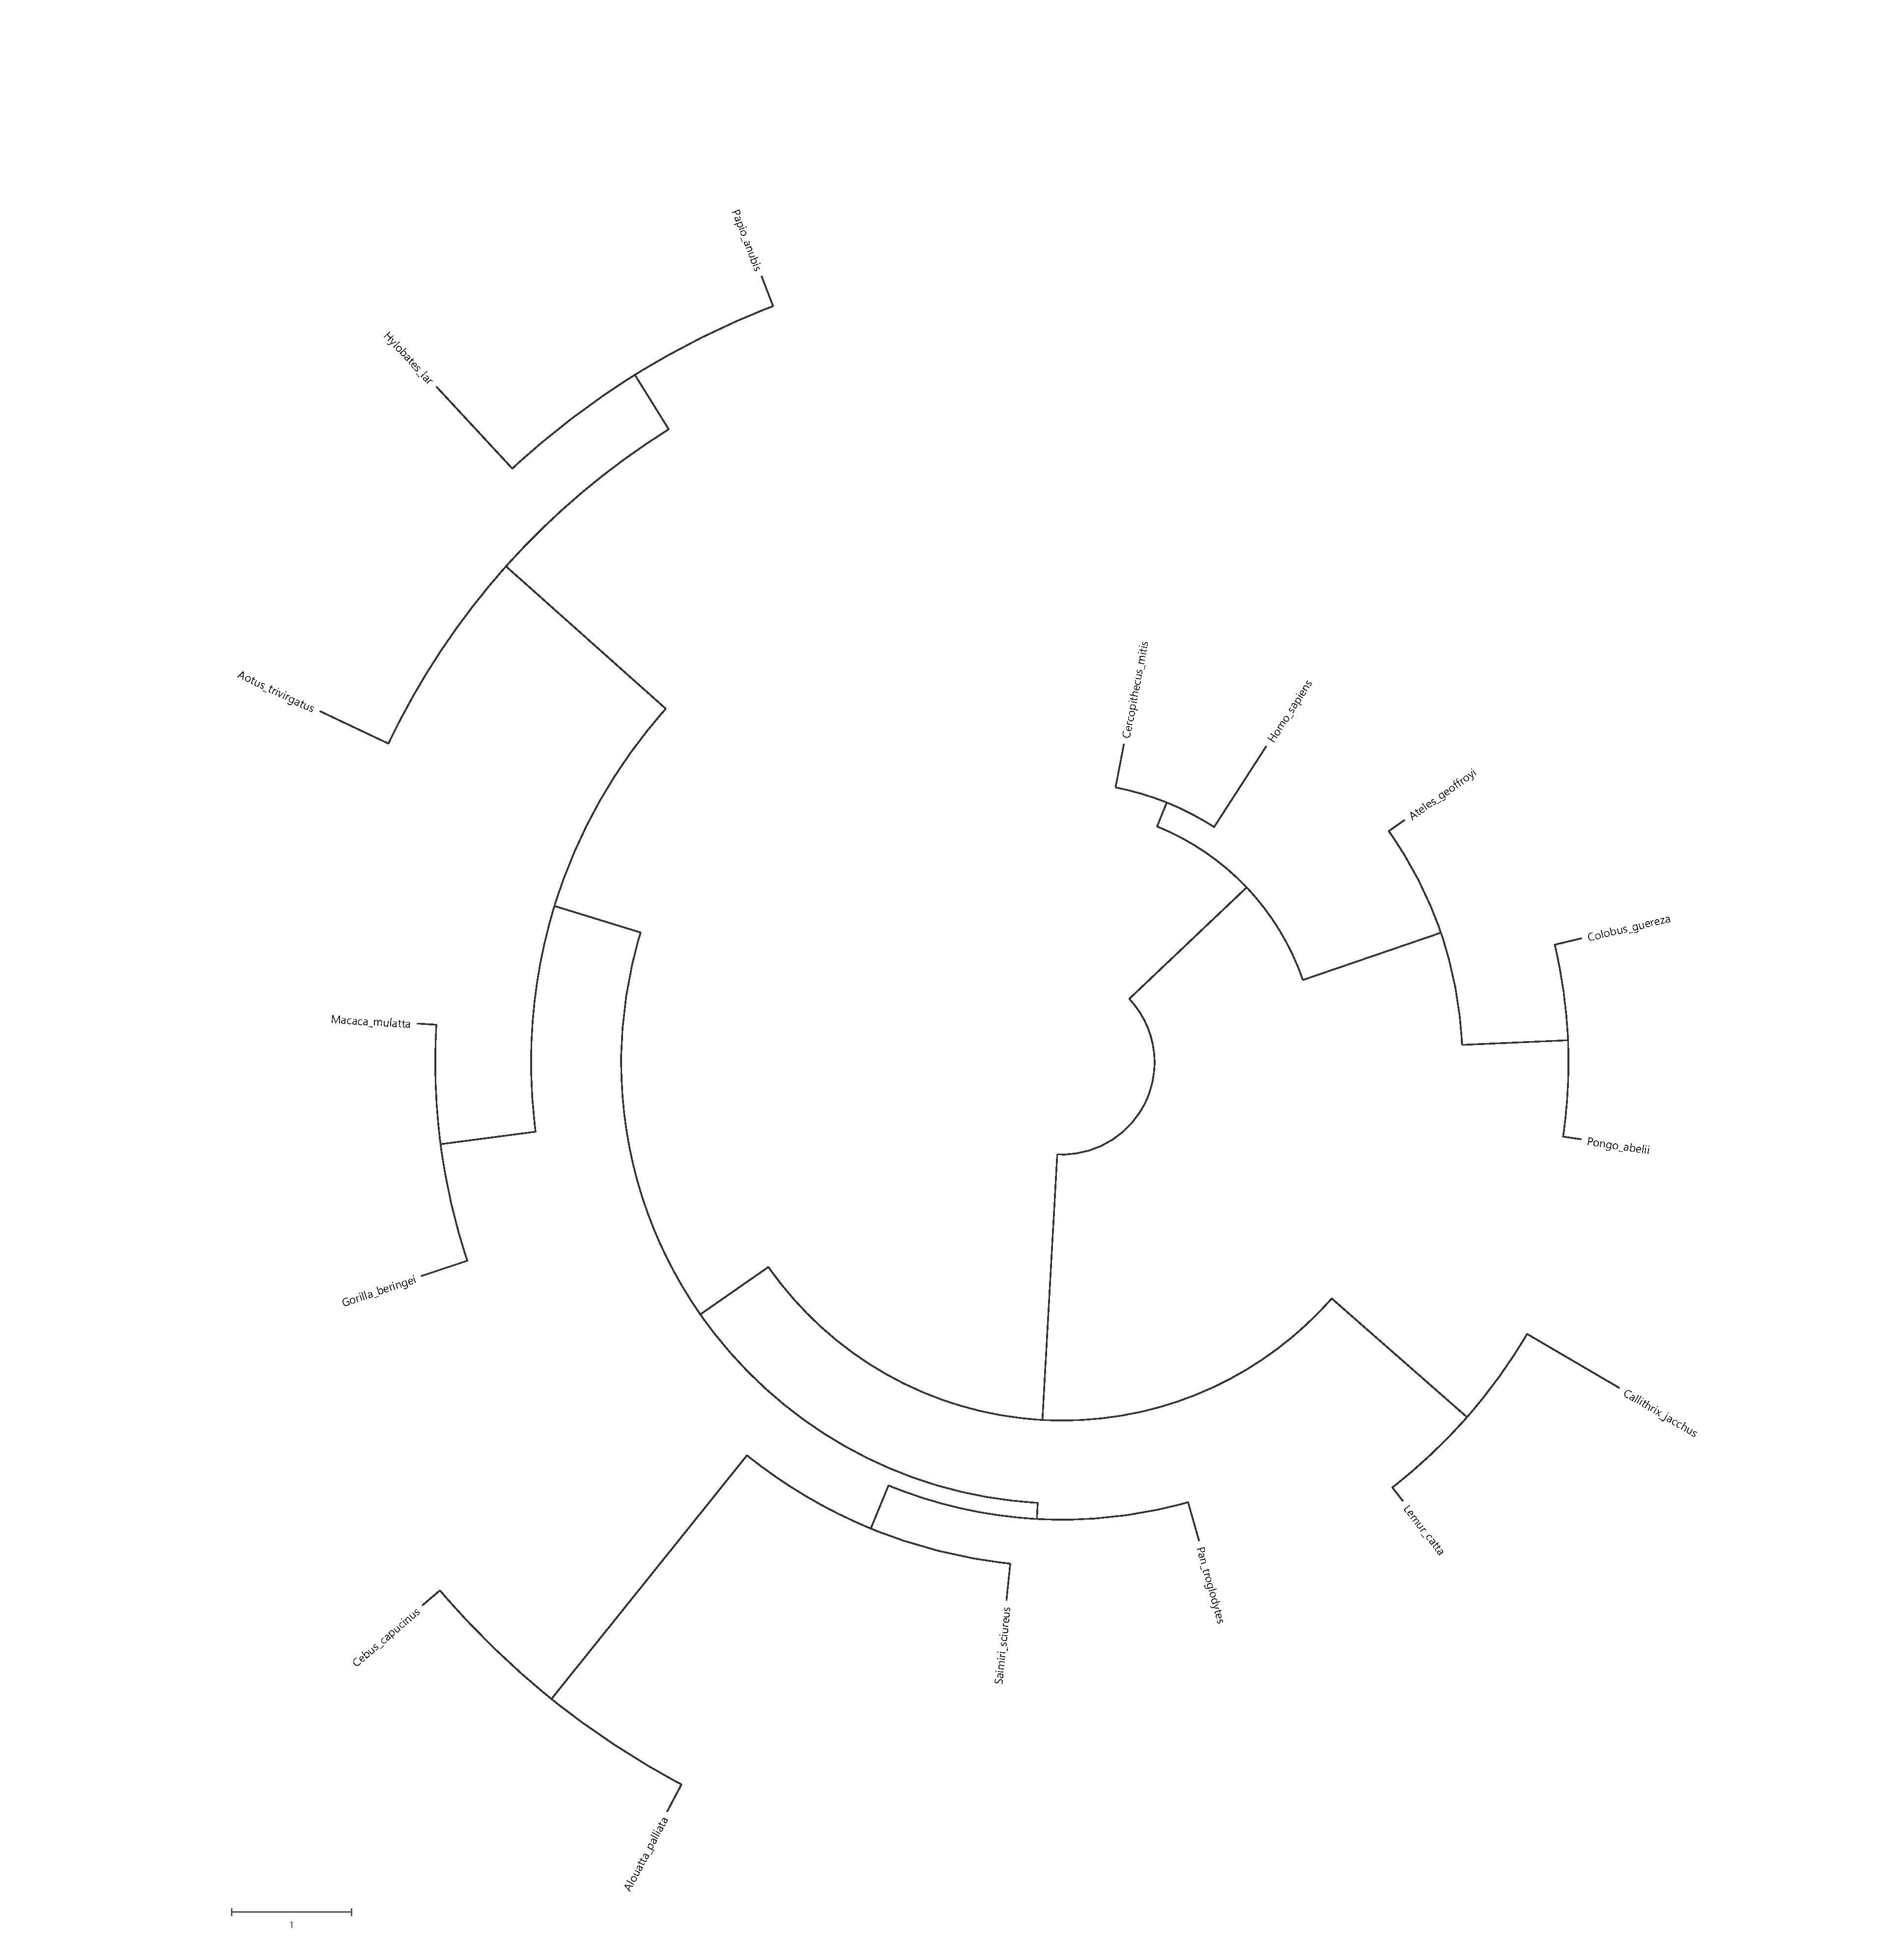
\includegraphics[width=0.72\linewidth]{layout-circular}
  \caption{A circular fan, the output of the second command above (shown
  without the track for clarity).}\label{fig:quickstart-circular}
\end{figure}

\section{The same thing in the application}

\begin{enumerate}
  \item Start the application:
    \begin{lstlisting}[language=bash]
makeyourtree-studio
    \end{lstlisting}
  \item \textbf{File \textbf{\textrightarrow} Open} and choose
        \cmd{examples/primates.nwk}. The tree appears immediately.
  \item Press \keys{3} to switch to a circular layout, or \keys{1} to go back to
        rectangular. The layout keys are \keys{1}--\keys{5}
        (Appendix~\ref{ch:shortcuts}).
  \item Press \keys{A} to align the tips and draw guide lines.
  \item \textbf{Annotate \textbf{\textrightarrow} Import Annotations}
        (\keys{Ctrl+I}) and choose \cmd{examples/primates\_region.mytrack}. A
        colour strip appears beside the tips, with a legend.
  \item \textbf{File \textbf{\textrightarrow} Export Figure} (\keys{Ctrl+E}).
        Choose SVG, PDF or PNG; the dialog predicts the pixel dimensions before
        you commit.
\end{enumerate}

Every step is undoable with \keys{Ctrl+Z}.

\section{A publication figure}

The example data includes a 24-tip bacterial tree with two annotation files.
Loading the tree and both tracks gives Figure~\ref{fig:combined-rectangular}:

\begin{lstlisting}[language=bash]
makeyourtree render examples/bacteria.nwk figure.svg --align-tips \
    --track examples/bacteria_resistance.mytrack \
    --track examples/bacteria_expression.mytrack
\end{lstlisting}

\galleryfig{combined-rectangular}{Three stacked tracks --- a categorical colour
strip, a diverging heatmap and a bar chart with a value axis --- beside a
rectangular phylogram. Tips are aligned and guide lines connect them to their
labels.}{1.0}

Switching that same figure to a circular layout requires changing one option, and
no track behaves differently:

\galleryfig{combined-circular}{The identical tracks and data in a circular
layout. The heatmap has become an annulus and the bars radiate outward; no track
code differs between this figure and Figure~\ref{fig:combined-rectangular}. This
is the band-space design of Section~\ref{sec:design} doing its work.}{0.85}

\section{From Python}

The same figure, reproducibly, from a script:

\begin{lstlisting}[language=Python]
from makeyourtree.io import load_tree
from makeyourtree.doc import Document
from makeyourtree.layout import LayoutParams, LayoutMode
from makeyourtree.scene import compose
from makeyourtree.render import render_svg
from makeyourtree.ops import midpoint_root, ladderize

tree = load_tree("examples/primates.nwk")
midpoint_root(tree).apply(tree)
ladderize(tree).apply(tree)

doc = Document(tree=tree,
               params=LayoutParams(mode=LayoutMode.CIRCULAR, arc=340))
with open("figure.svg", "w", encoding="utf-8") as fh:
    fh.write(render_svg(compose(doc)))
\end{lstlisting}

Chapter~\ref{ch:python} covers the API in full.

\section{Where to go next}

\begin{itemize}
  \item Chapter~\ref{ch:formats} --- what \app{} can read, and what it does with
        files that break their own specification.
  \item Chapter~\ref{ch:layouts} --- every layout mode, with figures.
  \item Chapter~\ref{ch:annotation} --- writing your own annotation files.
  \item Chapter~\ref{ch:tracks} --- the reference for all thirteen track types.
\end{itemize}


\part{Working with trees}
% SPDX-License-Identifier: MIT
\chapter{The interface}
\label{ch:interface}

\section{Layout of the window}

The window is a canvas surrounded by dockable panels. Every panel can be shown or
hidden from the \textbf{View} menu, and each has a shortcut
(Appendix~\ref{ch:shortcuts}).

\begin{center}
\begin{tabular}{@{}llp{0.52\linewidth}@{}}
\toprule
\textbf{Panel} & \textbf{Key} & \textbf{Purpose} \\
\midrule
Tree      & \keys{Alt+1} & The tree as a collapsible outline. Selecting a node here selects it on the canvas, and the reverse. \\
Style     & \keys{Alt+2} & Layout mode, branch mode, spacing, labels, theme. Most controls act immediately. \\
Tracks    & \keys{Alt+3} & The annotation stack. Reorder, hide, edit or remove tracks. \\
Search    & \keys{Ctrl+F} & Find taxa by name, with regular-expression support; matches are highlighted and selectable in bulk. \\
Inspector & \keys{Alt+4} & Everything known about the current selection: name, branch length, support, depth and any parsed annotations. \\
\bottomrule
\end{tabular}
\end{center}

\section{The canvas}

\subsection{Navigating}

\begin{itemize}
  \item \textbf{Zoom} with the mouse wheel. Zoom is anchored at the pointer, and
        it never re-runs the layout --- so zooming is instant regardless of tree
        size, and nothing shifts under the cursor.
  \item \textbf{Pan} by dragging with the middle button, or by dragging on empty
        canvas.
  \item \keys{Ctrl+0} fits the whole figure to the window;
        \keys{Ctrl+Shift+0} returns to actual size.
\end{itemize}

\subsection{Selecting}

Click a node to select it. Drag on empty canvas to rubber-band select a region.
\keys{Ctrl+Shift+A} extends the selection to the whole clade below the current
node, \keys{Ctrl+A} selects everything, and \keys{Esc} clears the selection.

Selection drives the tree operations in Chapter~\ref{ch:editing}: rerooting,
collapsing and pruning all act on what is selected.

\subsection{Context menu}

Right-clicking a node offers the operations that apply to it --- reroot here,
collapse, extract subtree, remove --- without going to the menu bar.

\section{The command palette}

\keys{Ctrl+P} opens a searchable list of every command in the application. It is
usually the fastest way to reach something whose menu location you cannot
remember, and it shows each command's keyboard shortcut alongside it, so it
doubles as a way to learn them.

The palette, the menus and the toolbar are all views of one registry of actions.
An action therefore cannot appear in one and be missing from another, and a
shortcut you rebind changes everywhere at once.

\section{Undo}

Every edit goes through a single command pipeline, so everything is undoable with
\keys{Ctrl+Z} and redoable with \keys{Ctrl+Shift+Z}. This includes operations
performed from the panels, not only those from the canvas.

Dragging a slider coalesces into a single history entry rather than one per pixel
of movement, so undo steps back over the whole drag.

\section{Themes}

\keys{Ctrl+T} switches between the light and dark themes. The theme belongs to
the figure, not merely to the screen: the composed scene carries its own
background colour, so an export made under the dark theme is dark in the file
too.

\galleryfig{feature-dark-theme}{The dark theme. Exports match the screen because
the background is part of the scene rather than a property of the window.}{0.9}

\section{Diagnostics}

When a file is loaded, anything \app{} had to interpret is recorded as a
diagnostic rather than discarded --- a duplicate tip name, a negative branch
length, an internal label that could be read either as a name or as a support
value. The status bar reports how many there were, and \keys{Ctrl+D} opens the
full list.

These are informational far more often than they are errors. A clean file
frequently produces one or two, and Chapter~\ref{ch:formats} explains the common
ones.

% SPDX-License-Identifier: MIT
\chapter{Tree file formats}
\label{ch:formats}

\section{What \app{} reads}

\begin{center}
\begin{tabular}{@{}llp{0.48\linewidth}@{}}
\toprule
\textbf{Format} & \textbf{Extensions} & \textbf{Notes} \\
\midrule
Newick   & \cmd{.nwk}, \cmd{.tree}, \cmd{.tre}, \cmd{.newick} &
  Full grammar: single-quoted labels with doubled-quote escapes, nested comments,
  branch lengths, support values. \\
NHX      & \cmd{.nhx} &
  New Hampshire eXtended. \cmd{[\&\&NHX:key=value]} annotations become typed node
  attributes. \\
NEXUS    & \cmd{.nex}, \cmd{.nexus} &
  Including \cmd{TRANSLATE} blocks and \cmd{[\&R]}/\cmd{[\&U]} rooting hints. \\
phyloXML & \cmd{.xml}, \cmd{.phyloxml} &
  Parsed with XML entity expansion disabled. \\
\bottomrule
\end{tabular}
\end{center}

Format is detected from the content, not only the extension, so a Newick tree
saved as \cmd{.txt} still loads. Pass \opt{--format} to the CLI to override
detection.

BEAST and FigTree \cmd{[\&key=value]} metacomments are also parsed, so trees from
those pipelines keep their posterior probabilities and rate annotations.

\section{Writing}

\app{} writes Newick, NEXUS and phyloXML. NHX is read but not written as a
separate format; NHX attributes are preserved on the nodes and can be written
back into Newick comments.

\section{Lenient parsing}

Real-world tree files violate their specifications routinely: unbalanced quotes,
duplicate tip labels, negative branch lengths, support values sitting where an
internal label should be. A parser that refuses such files is a parser you cannot
use on the files you actually have.

\app{} therefore records each recoverable problem as a \emph{diagnostic} and
carries on. Exceptions are reserved for input that cannot be interpreted at all.
Diagnostics are shown to you (\keys{Ctrl+D}) rather than hidden, so leniency does
not become silence.

\subsection{Diagnostics you are likely to see}

\begin{description}[style=nextline,leftmargin=0pt,labelindent=0pt,labelwidth=0pt]
  \item[\cmd{newick.internal-label-ambiguous}]
    Internal labels that parse as numbers. These are almost always bootstrap or
    posterior support values, so they are read as support. If yours are genuinely
    names, pass \cmd{internal\_labels='name'} through the API. This is the single
    most common diagnostic and it is informational.
  \item[\cmd{newick.duplicate-name}]
    Two tips share a name. Both are kept; annotation matching by name will attach
    to both, which is usually not what you want.
  \item[\cmd{newick.negative-length}]
    A negative branch length. By default these are treated as zero for layout
    purposes, which is controlled by \cmd{ignore\_negative\_lengths}.
  \item[\cmd{compose.approximate-band-space}]
    Raised when annotation tracks are drawn in an unrooted layout. See the
    warning in Section~\ref{sec:unrooted-tracks}.
\end{description}

\section{Security}

phyloXML is XML, and XML parsers are a classic vector for two attacks. \app{}
disables entity expansion entirely, which refuses both external-entity injection
(reading files off your disk) and entity-expansion denial of service (the
``billion laughs'' attack). A phyloXML file from an untrusted source cannot use
either against you.

\section{Large files}

Parsing is linear in tree size. A 100{,}000-tip Newick file parses in about
2.2~seconds and lays out in about 0.8~seconds on a normal workstation.

All traversals are iterative rather than recursive, which matters more than it
sounds: a deeply unbalanced tree --- the shape serially sampled sequence data
produces --- would exceed Python's recursion limit at a few thousand nodes under
a recursive implementation. \app{} handles a 50{,}000-node caterpillar tree
without difficulty.

The application remains responsive for trees of a few thousand tips. Beyond that,
switching layout mode takes several seconds during which the window does not
repaint; the work is not currently cancellable.

% SPDX-License-Identifier: MIT
\chapter{Layouts}
\label{ch:layouts}

There are five layout modes, selected with keys \keys{1}--\keys{5}, from the
Style panel, or with \opt{--mode} on the command line. Independently of the mode,
the \emph{branch mode} decides how the along-axis coordinate is derived.

\section{Branch modes}

\begin{center}
\begin{tabular}{@{}llp{0.5\linewidth}@{}}
\toprule
\textbf{Branch mode} & \textbf{Key} & \textbf{Along-axis coordinate} \\
\midrule
Phylogram              & \keys{Ctrl+1} & Cumulative branch length. Distances are meaningful. \\
Cladogram, aligned tips& \keys{Ctrl+2} & Depth, with every tip on the outer edge. Topology only. \\
Cladogram, by level    & \keys{Ctrl+3} & Node depth in levels. \\
\bottomrule
\end{tabular}
\end{center}

A phylogram shows evolutionary distance; a cladogram shows only branching order.
Use a cladogram when branch lengths are absent or meaningless, and say which you
used in the figure legend --- readers cannot tell by looking.

\section{Rectangular}

The default, and the right choice for most figures. Branch length runs along $x$,
tips are stacked down $y$.

\galleryfig{layout-rectangular-phylogram}{Rectangular phylogram. The scale bar at
the lower left gives the units of the horizontal axis.}{1.0}

\galleryfig{layout-rectangular-cladogram}{Rectangular cladogram with aligned
tips. Horizontal position now carries no distance information.}{1.0}

\section{Slanted}

Branches are drawn as straight diagonals rather than as right angles. Compact and
readable for small trees; harder to follow for large ones, because it is less
obvious which ancestor a branch descends from.

\galleryfig{layout-slanted}{Slanted layout.}{1.0}

\section{Circular}

Tips are placed around an arc. This is the layout that makes a large tree fit on
a page, and it is the natural home for multiple annotation rings.

Three options shape it:

\begin{center}
\begin{tabular}{@{}lll@{}}
\toprule
\textbf{Option} & \textbf{Default} & \textbf{Effect} \\
\midrule
\opt{arc}          & 350\textdegree & Angular span. 360\textdegree{} closes the circle. \\
\opt{inner\_radius}& 0.1            & Hole at the centre, as a fraction of the radius. \\
\opt{start\_angle} & $-90$\textdegree & Where the first tip sits. \\
\bottomrule
\end{tabular}
\end{center}

Leaving a small gap --- the default 350\textdegree{} --- makes it clear where the
tip order begins and ends. Closing to a full circle looks tidier but loses that
cue.

The gap does a second job that is easy to miss: it is the only place a track
caption can go. A rectangular tree captions its columns in a header row above
them and grows the page to fit; a fan has no room above its rings, so the
captions are written into the wedge the arc leaves open. Ask for several rings
with long names and the wedge fills up, at which point MakeYourTree reports the
captions it could not place rather than drawing them across the data. Widening
the gap --- \opt{arc} at 340\textdegree{} or 320\textdegree{} --- is the fix;
the legend names every track either way.

\galleryfig{layout-circular}{Circular fan with the default 350\textdegree{} arc.
Labels are rotated tangentially and flipped on the left-hand side so that none of
them is upside down.}{0.75}

\galleryfig{layout-circular-full}{A full 360\textdegree{} circle with a larger
inner radius.}{0.75}

\begin{quote}
\textbf{A gap you should not try to fix.} In a circular \emph{phylogram}, tips sit
at different radii because they are at different evolutionary distances from the
root. A ragged inner edge against an annotation ring is therefore correct, not a
bug. Turn on \textbf{Align tips} (\keys{A}) if you want the ring flush.
\end{quote}

\section{Radial}

Angle comes from tip order and radius from branch length, but the tree is drawn
outward from a central root without the concentric-arc branch style of the
circular mode.

\galleryfig{layout-radial}{Radial layout.}{0.75}

\section{Unrooted}

An unrooted layout makes no claim about which node is ancestral. Two algorithms
are available.

\begin{description}[style=nextline,leftmargin=0pt,labelindent=0pt,labelwidth=0pt]
  \item[Equal-angle] Felsenstein's original method. Each subtree receives a wedge
    proportional to the number of tips it contains. Fast and always planar.
  \item[Equal-daylight] Iteratively adjusts the wedges so the blank space between
    subtrees is evened out. Slower, usually easier to read.
\end{description}

Branch lengths are preserved exactly in both, and both are planar by
construction.

\galleryfig{layout-unrooted-equal-angle}{Unrooted, equal-angle.}{0.85}

\galleryfig{layout-unrooted-equal-daylight}{Unrooted, equal-daylight. The
subtrees are spread to even out the gaps between them.}{0.85}

\subsection{Annotation tracks in unrooted layouts}
\label{sec:unrooted-tracks}

\begin{quote}
\textbf{Known limitation.} An unrooted layout has no tip ordering along a line or
a circle, so band space has no faithful meaning in it. Tracks are currently drawn
as a column beside the figure, in tip order, \emph{aligned to nothing}. The
composition step emits the diagnostic
\cmd{compose.approximate-band-space} to record this, but the interface does not
yet present it prominently.

Do not use annotation tracks with an unrooted layout in a published figure
without saying so. Use a rooted layout instead.
\end{quote}

\section{Spacing and labels}

\begin{center}
\begin{tabular}{@{}lp{0.6\linewidth}@{}}
\toprule
\textbf{Setting} & \textbf{Effect} \\
\midrule
\opt{row\_spacing}   & Distance between adjacent tip rows. The main control over figure height. \\
\opt{width}, \opt{height} & Page size in scene units. \\
\opt{align\_tips}    & Flush all tip labels to a common edge. \\
\opt{guide\_lines}   & Dotted leaders from each tip to its label. Only meaningful with aligned tips. \\
\opt{show\_tip\_labels} & Turn tip labels off entirely --- often necessary above a few hundred tips. \\
\opt{max\_label\_width} & Truncate long labels with an ellipsis. \\
\bottomrule
\end{tabular}
\end{center}

\galleryfig{feature-align-tips}{Tips aligned with guide lines. This is almost
always what you want once an annotation track is attached, because it makes the
rows line up visually with the track cells.}{0.95}

% SPDX-License-Identifier: MIT
\chapter{Editing the tree}
\label{ch:editing}

Every operation in this chapter is undoable (\keys{Ctrl+Z}) and every one is also
available from the Python API (Chapter~\ref{ch:python}).

\section{Rooting}

Where the root sits changes what the figure claims. It does not change the tree's
topology in the unrooted sense, but it entirely changes which groups look
monophyletic, so it is worth being deliberate about.

\begin{center}
\begin{tabular}{@{}llp{0.48\linewidth}@{}}
\toprule
\textbf{Operation} & \textbf{Key} & \textbf{Description} \\
\midrule
Reroot here      & \keys{R} & Place the root on the branch above the selected node. \\
Midpoint root    & \keys{M} & Root at the midpoint of the longest tip-to-tip path. \\
Root on outgroup & \keys{Ctrl+Shift+R} & Root against a named taxon or set of taxa. \\
Unroot           & --- & Remove the root, collapsing it into a trifurcation. \\
\bottomrule
\end{tabular}
\end{center}

\textbf{Midpoint rooting} assumes a roughly constant rate of evolution across the
tree. It is a reasonable default when you have no outgroup, and a poor one when
rates vary substantially between lineages.

\textbf{Outgroup rooting} is preferable whenever you have a defensible outgroup,
because it encodes an actual biological hypothesis rather than an assumption
about rates.

\galleryfig{feature-midpoint-rooted}{The example tree after midpoint rooting.}{1.0}

\begin{quote}
\textbf{Branch lengths survive rerooting.} A branch length belongs to the
\emph{edge} between a node and its parent, and rerooting reverses the direction
of some edges. \app{} carries the lengths across those reversals, and the test
suite asserts that all pairwise tip-to-tip distances are unchanged by a reroot.
Rerooting is a change of viewpoint, not of data.
\end{quote}

\section{Ordering}

Reordering changes only the cross coordinate, so it can never alter a distance in
the figure.

\begin{center}
\begin{tabular}{@{}llp{0.48\linewidth}@{}}
\toprule
\textbf{Operation} & \textbf{Key} & \textbf{Description} \\
\midrule
Ladderize ascending  & \keys{L}       & Smaller subtrees first, giving the characteristic staircase. \\
Ladderize descending & \keys{Shift+L} & Larger subtrees first. \\
Rotate children      & \keys{Ctrl+R}  & Swap the order of the selected node's children. \\
\bottomrule
\end{tabular}
\end{center}

Ladderizing is almost always worth doing before exporting: it makes the branching
order far easier to follow, and costs nothing in accuracy.

\section{Collapsing}

Collapsing hides a clade's internal structure while keeping its position and
extent, which is the standard way to show a large tree without printing every
tip.

\keys{C} collapses or expands the selected node; \keys{Shift+C} expands
everything. A collapsed clade is drawn as a triangle whose depth reflects the
subtree it stands for.

\galleryfig{feature-collapsed-clade}{A collapsed clade. The triangle's size is
derived from the hidden subtree rather than being fixed, so the figure still
conveys how much was folded away.}{1.0}

The number of rows a collapsed clade occupies is configurable:
\opt{collapse\_rows\_mode} may be a square-root function of the subtree size (the
default, which keeps large clades from dominating), a fixed number of rows, or
proportional. \opt{collapse\_shape} selects the glyph.

\section{Pruning and extracting}

\begin{center}
\begin{tabular}{@{}llp{0.48\linewidth}@{}}
\toprule
\textbf{Operation} & \textbf{Key} & \textbf{Description} \\
\midrule
Remove selected taxa & \keys{Del}          & Delete tips and tidy away the internal nodes left dangling. \\
Extract subtree      & \keys{Ctrl+Shift+X} & Replace the document with the selected clade alone. \\
\bottomrule
\end{tabular}
\end{center}

When pruning removes a tip, the internal node above it may be left with a single
child. Such nodes are collapsed away, and the branch lengths on either side are
\emph{summed} rather than discarded, so the distances between the remaining tips
are preserved.

\section{Selecting}

Editing acts on the selection, so the selection tools matter.

\begin{itemize}
  \item Click a node, or drag a rubber band across several.
  \item \keys{Ctrl+Shift+A} extends the selection to the entire clade below the
        current node.
  \item The Search panel (\keys{Ctrl+F}) finds taxa by name or regular
        expression and can select every match at once --- the practical way to
        select a scattered group.
  \item \keys{Esc} clears the selection.
\end{itemize}


\part{Annotation}
% SPDX-License-Identifier: MIT
\chapter{The annotation format}
\label{ch:annotation}

Annotation lives in \cmd{.mytrack} files. One file describes one track: its type,
its data, and how it should look. The format is plain text and designed to be
hand-editable, generated by a script, or exported from a spreadsheet.

\section{A minimal file}

\begin{lstlisting}[language=mytrack]
#makeyourtree-annotation 1

[track]
type = color-strip
title = Biogeographic region

[columns]
names = region

[colors]
Neotropic   = #117733
Afrotropic  = #DDCC77
Palearctic  = #332288

[legend]
title = Region
show  = true

[data]
Homo_sapiens        Palearctic
Pan_troglodytes     Afrotropic
Aotus_trivirgatus   Neotropic
\end{lstlisting}

The first line is the magic marker and is required. Everything after it is a
series of \cmd{[section]} blocks.

\section{Sections}

\begin{center}
\begin{tabular}{@{}lp{0.62\linewidth}@{}}
\toprule
\textbf{Section} & \textbf{Contents} \\
\midrule
\cmd{[track]}   & \cmd{type} (required), \cmd{title}, and \cmd{match}. \\
\cmd{[options]} & Appearance settings for this track type. Chapter~\ref{ch:tracks} lists them per type. \\
\cmd{[columns]} & \cmd{names = a, b, c} --- the column headers, used in legends and axis labels. \\
\cmd{[colors]}  & Explicit colour per category, overriding the automatic palette. \\
\cmd{[legend]}  & \cmd{title}, \cmd{show}, \cmd{order}. \\
\cmd{[data]}    & One row per node: a key, then one value per column. \\
\bottomrule
\end{tabular}
\end{center}

Only \cmd{[track]} with a \cmd{type}, and \cmd{[data]}, are strictly required.

\section{The data section}

Each row begins with a key that identifies a node, followed by one value per
column. Three separators are recognised, tried in this order:

\begin{enumerate}
  \item a tab,
  \item a comma,
  \item a run of two or more spaces.
\end{enumerate}

The last of these means a column-aligned table pasted out of a terminal works
without editing. A single space never separates fields, so taxon names may
contain spaces.

Quoting follows the CSV convention of RFC~4180: wrap a field in double quotes,
and write a literal quote inside it twice.

\subsection{Matching rows to nodes}

By default keys are matched against tip names. \cmd{match = all} in the
\cmd{[track]} section allows internal nodes to match too, which is what
\cmd{clade-range} needs.

If the first data line begins with one of \cmd{id}, \cmd{key}, \cmd{name},
\cmd{node}, \cmd{label}, \cmd{taxon}, \cmd{tip} or \cmd{leaf}, it is treated as a
header row rather than as data.

Rows that match nothing are not silently dropped: they are reported, and the
application's import dialog shows a match report before you commit, so you find
out about a naming mismatch before it becomes a wrong figure.

\subsection{Missing is not zero}

An empty field, or a single \cmd{-}, means \emph{no value}. The track draws a gap
there. This is deliberate and it matters: a zero would be a fabricated
measurement, and a reader cannot tell a fabricated zero from a real one.

\section{Importing a spreadsheet}

You do not have to write \cmd{.mytrack} files by hand. \textbf{Annotate
\textbf{\textrightarrow} Import Annotations} (\keys{Ctrl+I}) reads CSV and
tab-separated files directly. The wizard lets you choose the track type, say which
column holds the node key, and see how many rows matched before anything is
added.

The usual workflow is to keep your data in a spreadsheet, export it as CSV, and
import it. Save the resulting project (\cmd{.mytree}) and the track travels with
it.

\section{Leniency and round-tripping}

Unknown sections and unknown keys are \emph{kept}, not discarded, and recorded as
diagnostics. If a future version writes a key this one does not understand, your
file survives a load-and-save cycle unharmed.

A table written by \app{} and read back is identical to the original. The writer
quotes any field whose bare form would be re-read as something else --- a number,
a \cmd{-}, or a boolean.

The only genuinely fatal error is a file that declares no track type.

\section{Colours}

Colours may be given as \cmd{\#RRGGBB}, \cmd{\#RGB}, \cmd{rgb()} or
\cmd{rgba()}. Bare colour \emph{names} are deliberately not accepted in the
\cmd{[colors]} section, because \cmd{red} is far more often a category label than
a colour request --- accepting it would silently merge a category with its own
swatch.

When no explicit colours are given, categories are assigned from a
colour-vision-safe palette. Twenty-one palettes are available, including the
Paul Tol sets, Okabe--Ito, and the perceptually uniform \cmd{viridis} family.
Prefer these over a hand-picked rainbow: roughly 1 in 12 men has a red--green
colour vision deficiency, and a figure they cannot read is a figure that fails.

% SPDX-License-Identifier: MIT
\chapter{Track reference}
\label{ch:tracks}

Thirteen track types are available. Each is described below with its data shape,
its most useful options and a figure produced by \app{}.

Every track works in every rooted layout mode without configuration, because
tracks are written in band space (Section~\ref{sec:design}). The one exception is
unrooted layouts, where alignment is not meaningful --- see
Section~\ref{sec:unrooted-tracks}.

\section{Options common to all tracks}

\begin{center}
\begin{tabular}{@{}llp{0.52\linewidth}@{}}
\toprule
\textbf{Option} & \textbf{Default} & \textbf{Effect} \\
\midrule
\opt{thickness}    & varies & How much room the track takes, outward from the tree. \\
\opt{gap\_before}  & --- & Space between this track and the previous one. \\
\opt{opacity}      & 1.0 & Whole-track transparency. \\
\opt{border\_color}, \opt{border\_width} & --- & Outline around drawn elements. \\
\opt{show\_title}  & true & Draw the track title beside the stack. \\
\bottomrule
\end{tabular}
\end{center}

Tracks are drawn in the order they appear in the Tracks panel, stacking outward.
Drag to reorder.

% =====================================================================
\section{Categorical tracks}

\subsection{Colour strip}

One categorical value per tip, drawn as a band of colour. The most common
annotation of all: host, region, lineage, clinical outcome.

\textbf{Data:} one column of category labels.\\
\textbf{Key options:} \opt{colors} (explicit category colours), \opt{palette},
\opt{thickness}, \opt{merge\_runs}, \opt{color\_branches}, \opt{color\_labels},
\opt{margin}.

\opt{color\_branches} and \opt{color\_labels} propagate the category colour onto
the tree itself, which is often more readable than a separate band.
\opt{merge\_runs} joins adjacent tips of the same category into one block.

\galleryfig{track-color-strip}{Colour strip with an explicit colour-vision-safe
palette and a legend.}{0.95}

\subsection{Binary matrix}

Presence and absence across several features --- gene content, resistance
profiles, trait matrices.

\textbf{Data:} one column per feature; values \cmd{1} (present), \cmd{0} (absent)
and \cmd{-1} or empty (unknown).\\
\textbf{Key options:} \opt{shape} (\cmd{square}, \cmd{circle}, and others),
\opt{cell\_size}, \opt{column\_colors}, \opt{column\_shapes},
\opt{show\_absent}, \opt{label\_rotation}.

Present, absent and unknown are three distinct states, and the track draws them
differently. Do not encode unknown as absent.

\galleryfig{track-binary-matrix}{Binary matrix over six genes for 24 strains.}{0.95}

\subsection{Symbols}

A shape per node, its size and colour driven by data.

\textbf{Data:} typically one column for colour and one for size.\\
\textbf{Key options:} \opt{color\_column}, \opt{size\_column},
\opt{shape}, \opt{shape\_column}, \opt{size\_mode}, \opt{min\_size},
\opt{max\_size}, \opt{at\_nodes}.

\begin{quote}
\opt{size\_mode} defaults to \cmd{sqrt}, so the drawn \emph{area} is proportional
to the value. This is the correct choice: readers judge a symbol by its area, and
a radius-linear encoding exaggerates large values by roughly the square.
\cmd{linear} is available for compatibility with tables authored against a
radius-linear tool, but it is a decision you should make knowingly.
\end{quote}

\galleryfig{track-symbols}{Symbols coloured by habitat and sized by count.}{0.95}

% =====================================================================
\section{Continuous tracks}

\subsection{Gradient}

A single continuous value per tip as one colour ramp. Compact --- useful when you
have many tracks and little room.

\textbf{Data:} one numeric column.\\
\textbf{Key options:} \opt{color\_min}, \opt{color\_mid}, \opt{color\_max},
\opt{use\_mid}, \opt{min\_value}, \opt{max\_value}, \opt{stops},
\opt{missing\_color}.

\galleryfig{track-gradient}{Gradient track.}{0.95}

\subsection{Heatmap}

A matrix of continuous values: expression across conditions, abundance across
samples, distance to a reference.

\textbf{Data:} one column per condition.\\
\textbf{Key options:} \opt{cell\_size}, \opt{cell\_gap}, \opt{normalize}
(\cmd{global}, \cmd{row}, \cmd{column}), \opt{color\_min}, \opt{color\_mid},
\opt{color\_max}, \opt{use\_mid}, \opt{cluster\_columns}, \opt{cluster\_rows},
\opt{show\_values}, \opt{column\_labels}.

\begin{quote}
\textbf{There is no \opt{palette} option here} --- the ramp is set by
\opt{color\_min}, \opt{color\_mid} and \opt{color\_max}. For data with a
meaningful zero, such as log fold change, use a \emph{diverging} ramp centred on
white and set \opt{use\_mid}; a sequential ramp will hide the sign.
\opt{normalize} controls whether the scale is computed over the whole matrix, per
row, or per column --- and choosing wrongly is an easy way to mislead, so say
which you used.
\end{quote}

\galleryfig{track-heatmap}{Heatmap with a diverging blue--white--red ramp,
normalised globally.}{0.95}

% =====================================================================
\section{Chart tracks}

\subsection{Bar chart}

\textbf{Data:} one numeric column, or several for a stacked or grouped chart.\\
\textbf{Key options:} \opt{stack}, \opt{color}, \opt{colors}, \opt{axis},
\opt{axis\_ticks}, \opt{value\_min}, \opt{value\_max}, \opt{zero\_based},
\opt{bar\_gap}, \opt{series\_gap}.

Leave \opt{zero\_based} on unless you have a specific reason: a truncated bar axis
misrepresents ratios, which is the most common way a bar chart lies.

\galleryfig{track-bar-chart}{Bar chart with a value axis.}{0.95}

\galleryfig{track-bar-stacked}{Stacked bar chart showing composition per tip.}{0.95}

\subsection{Box plot}

Distribution per tip, rather than a single value.

\textbf{Data:} either raw replicate values (\opt{source} = \cmd{raw}) or
pre-computed five-number summaries.\\
\textbf{Key options:} \opt{source}, \opt{whisker\_factor}, \opt{show\_outliers},
\opt{box\_height}, \opt{box\_color}, \opt{median\_color}, \opt{axis}.

\galleryfig{track-box-plot}{Box plots computed from seven raw replicates per
tip.}{0.95}

\subsection{Pie chart}

Part-to-whole composition at each node.

\textbf{Data:} one column per slice; values need not sum to 1.\\
\textbf{Key options:} \opt{radius}, \opt{donut}, \opt{colors},
\opt{size\_column}, \opt{at\_nodes}, \opt{start\_angle}.

\opt{donut} converts the pie to a ring, and \opt{size\_column} scales each pie by
a further variable --- useful for showing both composition and total.

\galleryfig{track-pie-chart}{Donut charts at each tip.}{0.95}

\subsection{Line chart}

A small time series or profile per tip.

\textbf{Data:} one column per time point.\\
\textbf{Key options:} \opt{zero\_line}, \opt{area}, \opt{area\_opacity},
\opt{show\_dots}, \opt{dot\_radius}, \opt{line\_width}, \opt{y\_range},
\opt{value\_min}, \opt{value\_max}.

Set \opt{y\_range} explicitly when comparing tips: with a per-row range, two
rows of very different magnitude look identical.

\galleryfig{track-line-chart}{Line charts with a zero line and shaded area.}{0.95}

% =====================================================================
\section{Structural tracks}

\subsection{Clade range}

A shaded, labelled band behind an entire clade. The way to name and highlight
groups.

\textbf{Data:} keyed by \emph{internal} node, with a colour and a label. Requires
\cmd{match = all}.\\
\textbf{Key options:} \opt{show\_labels}, \opt{label\_position},
\opt{label\_rotation}, \opt{cover}, \opt{extend}, \opt{row\_shrink},
\opt{inner\_offset}.

Drawn beneath the branches so the topology stays legible through the wash.

\galleryfig{track-clade-range}{Clade ranges naming three groups.}{0.95}

\subsection{Domain architecture}

Protein features drawn to scale along a backbone --- domains, motifs,
transmembrane segments.

\textbf{Data:} a length column, then one column per feature, each formatted
\cmd{start|end|shape|colour|label}.\\
\textbf{Key options:} \opt{length\_column}, \opt{feature\_height},
\opt{backbone\_height}, \opt{show\_labels}, \opt{min\_feature\_width}.

Features are positioned in sequence coordinates, so proteins of different lengths
are drawn on a common scale and are directly comparable.

\galleryfig{track-domain-architecture}{Domain architecture. Features are drawn at
their true sequence positions along each backbone.}{0.95}

\subsection{Text labels}

Arbitrary text beside each tip, independent of the tip name.

\textbf{Data:} one column of strings.\\
\textbf{Key options:} \opt{size}, \opt{color}, \opt{color\_column}, \opt{align},
\opt{bold}, \opt{italic}, \opt{max\_width}, \opt{ellipsize},
\opt{rotate\_with\_layout}.

\galleryfig{track-text-labels}{Text labels carrying notes independent of the tip
names.}{0.9}

\subsection{Connections}

Curved links between arbitrary node pairs: gene transfer, recombination, host
jumps, co-occurrence.

\textbf{Data:} each row gives two node names, and optionally a weight, a colour
and a label.\\
\textbf{Key options:} \opt{bow}, \opt{width\_scale}, \opt{min\_width},
\opt{max\_width}, \opt{show\_labels}, \opt{color}, \opt{anchor}.

This track is unusual in two ways: it annotates a \emph{relation} rather than a
node, and it consumes no thickness at all. Links are drawn over the tree body,
beneath the branches, so a dense bundle never obscures the topology it is drawn
against.

\galleryfig{track-connections}{Connections between four pairs of tips, with width
scaled by weight.}{0.95}

% =====================================================================
\section{Stacking tracks}

Tracks stack outward in panel order, and any combination may be used together.
Figure~\ref{fig:feature-large-tree} shows a categorical strip and a heatmap
around a 24-tip tree.

\galleryfig{feature-large-tree}{A colour strip and a heatmap wrapped around a
circular layout with aligned tips.}{0.8}


\part{Output and automation}
% SPDX-License-Identifier: MIT
\chapter{Exporting and projects}
\label{ch:export}

\section{Exporting a figure}

\textbf{File \textbf{\textrightarrow} Export Figure} (\keys{Ctrl+E}) writes the
current figure. Three formats are available.

\begin{center}
\begin{tabular}{@{}llp{0.48\linewidth}@{}}
\toprule
\textbf{Format} & \textbf{Kind} & \textbf{Use it for} \\
\midrule
SVG & Vector & Journal submission, and any figure you intend to edit afterwards in a vector editor. \\
PDF & Vector & Journal submission, and inclusion in \LaTeX{} documents. \\
PNG & Raster & Slides, web pages, quick sharing. \\
\bottomrule
\end{tabular}
\end{center}

\textbf{Prefer a vector format wherever it is accepted.} A vector figure has no
resolution: it stays sharp at any magnification and in print. Use PNG only where
raster is required.

For PNG, a scale factor multiplies the figure's natural size. The export dialog
predicts the resulting pixel dimensions before you commit, so you can hit a
journal's minimum resolution without guessing. A scale of 2--4 is typical for
print.

\section{Sizes and resolution}

A scene unit is a \textbf{PostScript point}, 1/72 inch, and every output honours
that. An SVG carries \cmd{pt} on its \cmd{width} and \cmd{height}, a PDF page is
measured in points, and a PNG multiplies by \opt{dpi}/72. The consequence worth
knowing is that the same figure exported as SVG and as PDF is the \emph{same
physical size}, so the two can be swapped in a manuscript without anything
moving.

For raster output the DPI box and the pixel boxes are two views of one number:
changing either updates the other. 300\,dpi is the usual journal minimum and
600\,dpi is sometimes required. The pixel size predicted in the dialog is
exactly what lands on disk.

The command line offers the same controls, plus physical units and named page
sizes --- see Section~\ref{ch:cli}.

\section{What you see is what you get}

The canvas and all three exporters consume an identical description of the
figure. There is no separate rendering path for export, so a figure cannot differ
between the screen and the file. This includes the theme: a figure composed under
the dark theme exports dark.

\section{Projects}

A project file (\cmd{.mytree}) holds the tree, the layout settings, the theme and
every annotation track, so reopening it restores the figure exactly as you left
it.

\begin{center}
\begin{tabular}{@{}ll@{}}
\toprule
\textbf{Action} & \textbf{Key} \\
\midrule
Save          & \keys{Ctrl+S} \\
Save As       & \keys{Ctrl+Shift+S} \\
Open Project  & \keys{Ctrl+Shift+O} \\
\bottomrule
\end{tabular}
\end{center}

A project is a container carrying a manifest plus the tree and annotation data.
Because the tracks travel inside it, a project is self-contained: you can move it
to another machine and it will open with its annotations intact, without the
original \cmd{.mytrack} files alongside.

Projects are treated as untrusted input on load, in the same way tree files are:
a project arriving by email or download is parsed defensively rather than
trusted.

\section{Preparing a figure for publication}

A short checklist, in the order that tends to work:

\begin{enumerate}
  \item \textbf{Root deliberately.} Outgroup rooting if you have an outgroup,
        midpoint otherwise --- and say which in the caption
        (Chapter~\ref{ch:editing}).
  \item \textbf{Ladderize} (\keys{L}). It costs nothing and makes branching
        order far easier to follow.
  \item \textbf{Align tips} (\keys{A}) once you have annotation tracks, so rows
        line up with track cells.
  \item \textbf{Check the colours.} Prefer the built-in colour-vision-safe
        palettes over a hand-picked rainbow.
  \item \textbf{Say what the branch lengths mean}, or turn them off with a
        cladogram if they are meaningless. Readers cannot tell by looking.
  \item \textbf{State the support values} shown, and what they are --- bootstrap
        percentages and posterior probabilities look identical and mean quite
        different things.
  \item \textbf{Export vector} (SVG or PDF).
  \item \textbf{Save the project} alongside the figure, so the figure can be
        regenerated or corrected later.
\end{enumerate}

For a figure that must be reproducible from a pipeline rather than from a saved
project, generate it from a script instead --- Chapters~\ref{ch:cli}
and~\ref{ch:python}.

% SPDX-License-Identifier: MIT
\chapter{The command line}
\label{ch:cli}

The \cmd{makeyourtree} command needs no GUI toolkit, so it works on a headless
server, in a container and in continuous integration. It has four subcommands.

\begin{lstlisting}[language=bash]
makeyourtree --help
makeyourtree <command> --help
\end{lstlisting}

\section{\cmd{info} --- summarise a tree}

\begin{lstlisting}[language=bash]
makeyourtree info examples/primates.nwk
\end{lstlisting}

Reports the detected format, tip and node counts, whether the tree is rooted and
binary, its height, the longest root-to-tip distance, whether branch lengths and
support values are present, and whether it is ultrametric. Any diagnostics from
parsing are printed first.

\begin{center}
\begin{tabular}{@{}ll@{}}
\toprule
\textbf{Option} & \textbf{Effect} \\
\midrule
\opt{-{}-format} & Override format detection. \\
\opt{-{}-json}   & Emit a JSON object instead of the text summary. \\
\bottomrule
\end{tabular}
\end{center}

\opt{--json} is the one to use from a script; the text layout is for humans and
may change.

\section{\cmd{convert} --- change format}

\begin{lstlisting}[language=bash]
makeyourtree convert tree.nex tree.xml
makeyourtree convert tree.nwk out.nex --format nexus
\end{lstlisting}

The output format is inferred from the extension unless \opt{--format} says
otherwise. \opt{--input-format} overrides detection on the input. Newick, NEXUS
and phyloXML can be written; all four formats can be read.

\section{\cmd{render} --- write a figure}

The subcommand that does the most work. It writes SVG, PDF or PNG.

\begin{lstlisting}[language=bash]
makeyourtree render examples/primates.nwk figure.svg \
    --mode circular --branch-mode phylogram \
    --ladderize asc --align-tips \
    --track examples/primates_region.mytrack \
    --theme light --width 1200
\end{lstlisting}

\begin{center}
\begin{tabular}{@{}lp{0.56\linewidth}@{}}
\toprule
\textbf{Option} & \textbf{Effect} \\
\midrule
\opt{-{}-mode}        & \cmd{rectangular}, \cmd{slanted}, \cmd{circular}, \cmd{radial}, \cmd{unrooted}. \\
\opt{-{}-branch-mode} & \cmd{phylogram}, \cmd{cladogram-aligned}, \cmd{cladogram-level}. \\
\opt{-{}-width}, \opt{-{}-height} & Page size, with an optional unit: \cmd{180mm}, \cmd{7in}, \cmd{900pt}, \cmd{1200px}. A bare number is points. \\
\opt{-{}-output-format} & \cmd{svg}, \cmd{pdf} or \cmd{png}. Defaults to whatever the output extension says. \\
\opt{-{}-dpi}         & Resolution for raster output, default 300. Ignored by the vector formats. \\
\opt{-{}-page}        & A named page size instead of \opt{-{}-width}/\opt{-{}-height}. \\
\opt{-{}-landscape}   & Swap the axes of \opt{-{}-page}. \\
\opt{-{}-row-spacing} & Distance between adjacent tip rows. \\
\opt{-{}-ladderize}   & \cmd{asc} or \cmd{desc}, applied before layout. \\
\opt{-{}-align-tips}  & Flush tip labels and draw guide lines. \\
\opt{-{}-no-tip-labels} & Omit tip labels entirely. \\
\opt{-{}-track FILE}  & Attach an annotation file. Repeatable; tracks stack in the order given. \\
\opt{-{}-theme}       & \cmd{light} or \cmd{dark}. \\
\opt{-{}-format}      & Override format detection on the input. \\
\bottomrule
\end{tabular}
\end{center}

\subsection{Choosing the format}

The output extension picks the format, so the common case needs no flag:

\begin{lstlisting}[language=bash]
makeyourtree render tree.nwk figure.svg     # vector
makeyourtree render tree.nwk figure.pdf     # vector
makeyourtree render tree.nwk figure.png     # raster, 300 dpi
\end{lstlisting}

\opt{--output-format} overrides it when the extension is missing or misleading.

\begin{quote}
\textbf{PNG and PDF need the desktop extra.} Rasterising requires Qt, and the
\cmd{makeyourtree} library deliberately does not depend on it. With the library
alone SVG works, and asking for a PNG tells you to run
\cmd{pip install 'makeyourtree[studio]'} rather than failing with a traceback.
SVG needs nothing beyond the library and is a fine choice for a headless
pipeline.
\end{quote}

\subsection{Resolution}

\opt{--dpi} sets pixels per inch for raster output. The default of 300 is the
usual journal minimum; 600 is asked for by some, and 150 is plenty for a slide.

\begin{lstlisting}[language=bash]
makeyourtree render tree.nwk figure.png --dpi 600
\end{lstlisting}

It does nothing to SVG or PDF, which have no pixels. A vector figure is sharp at
any size, which is why it is the better choice wherever the destination takes
one.

\subsection{Physical size}

\opt{--width} and \opt{--height} take a unit --- \cmd{mm}, \cmd{cm}, \cmd{in},
\cmd{pt} or \cmd{px}. A bare number is points, so an existing
\cmd{--width 900} keeps its old meaning.

\begin{lstlisting}[language=bash]
makeyourtree render tree.nwk figure.pdf --width 180mm
makeyourtree render tree.nwk figure.png --width 7in --dpi 600
makeyourtree render tree.nwk figure.pdf --page a4 --landscape
\end{lstlisting}

\begin{center}
\begin{tabular}{@{}ll@{}}
\toprule
\textbf{Preset} & \textbf{Size} \\
\midrule
\cmd{a5}, \cmd{a4}, \cmd{a3} & ISO paper, portrait \\
\cmd{letter}, \cmd{legal}, \cmd{tabloid} & US paper, portrait \\
\cmd{column} & A single journal column; height left to the figure \\
\cmd{wide-column} & A double column; height left to the figure \\
\bottomrule
\end{tabular}
\end{center}

An explicit \opt{--width} or \opt{--height} overrides the preset on that axis,
so a preset can serve as a starting point.

\begin{quote}
\textbf{A requested size is a floor, never a crop.} If the figure needs more room
than you asked for --- long tip labels are the usual reason --- it is drawn at
its natural size and nothing is cut off. The command says so on standard error
rather than leaving you to discover it later. To make a figure genuinely fit,
shorten or drop the tip labels, reduce \opt{--row-spacing}, or scale it down
when you place it.
\end{quote}

Every run reports what it produced, so the size is discoverable without opening
the file:

\begin{lstlisting}[language=bash]
$ makeyourtree render examples/primates.nwk figure.png --dpi 300
figure.png  4264 x 1410 px at 300 dpi (361.0mm x 119.3mm)
\end{lstlisting}

\cmd{-q} before the subcommand silences it.

\opt{--track} may be given more than once, which is how you build a multi-track
figure non-interactively:

\begin{lstlisting}[language=bash]
makeyourtree render examples/bacteria.nwk figure.svg --align-tips \
    --track examples/bacteria_resistance.mytrack \
    --track examples/bacteria_expression.mytrack
\end{lstlisting}

\section{\cmd{reroot} --- place a new root}

\begin{lstlisting}[language=bash]
makeyourtree reroot tree.nwk rooted.nwk --midpoint
makeyourtree reroot tree.nwk rooted.nwk --outgroup Homo_sapiens,Pan_troglodytes
\end{lstlisting}

Exactly one of \opt{--midpoint} or \opt{--outgroup} is required.
\opt{--outgroup} takes a comma-separated list of taxon names. The output format
follows the extension unless \opt{--output-format} says otherwise.

Pairwise tip-to-tip distances are unchanged by rerooting.

\section{Scripting}

The commands compose in a pipeline. To convert, reroot and render a directory of
trees:

\begin{lstlisting}[language=bash]
for f in trees/*.nwk; do
  base=$(basename "$f" .nwk)
  makeyourtree reroot "$f" "rooted/$base.nwk" --midpoint
  makeyourtree render "rooted/$base.nwk" "figures/$base.svg" \
      --mode circular --ladderize asc --align-tips
done
\end{lstlisting}

Every subcommand exits non-zero on failure, so \cmd{set -e} behaves as expected.

For anything more elaborate --- conditional styling, computed annotations,
tracks built from data you already have in memory --- use the Python API in
Chapter~\ref{ch:python} rather than shelling out repeatedly.

% SPDX-License-Identifier: MIT
\chapter{The Python API}
\label{ch:python}

The \cmd{makeyourtree} package imports no GUI toolkit, so everything in this
chapter runs in a script, a notebook, a container or a CI job.

\section{Loading and inspecting}

\begin{lstlisting}[language=Python]
from makeyourtree.io import load_tree, save_tree

tree = load_tree("examples/primates.nwk")

print(len(tree.nodes))
print([n.name for n in tree.nodes if not n.children])
print(tree.rooted)
\end{lstlisting}

\cmd{load\_tree} detects the format from the content. Pass \cmd{format=} to
override it. \cmd{load\_trees} reads a multi-tree file.

\subsection{Diagnostics}

Parsing problems are collected rather than raised. To see them, pass a sink:

\begin{lstlisting}[language=Python]
from makeyourtree.core.diagnostics import DiagnosticSink

sink = DiagnosticSink()
tree = load_tree("messy.nwk", sink=sink)
for d in sink:
    print(d.code, d.message)
\end{lstlisting}

\section{Traversal}

\begin{quote}
\textbf{Never recurse over a tree.} A deeply unbalanced tree of 100{,}000 tips
has a path length of 100{,}000, and Python's recursion limit is 1{,}000. Use the
iterative traversals in \cmd{makeyourtree.core.traversal}; every traversal inside
\app{} is iterative for exactly this reason.
\end{quote}

\begin{lstlisting}[language=Python]
from makeyourtree.core import traversal

for node in traversal.preorder(tree.root):
    ...
for node in traversal.postorder(tree.root):
    ...
\end{lstlisting}

\section{Operations}

Operations return a \emph{command} rather than mutating immediately, which is
what makes them undoable in the application. From a script, apply it at once:

\begin{lstlisting}[language=Python]
from makeyourtree.ops import (midpoint_root, outgroup_root, ladderize,
                              rotate, collapse, prune, extract_subtree, unroot)

midpoint_root(tree).apply(tree)
ladderize(tree, ascending=True).apply(tree)
\end{lstlisting}

To keep an undo history, use a \cmd{CommandStack}:

\begin{lstlisting}[language=Python]
from makeyourtree.ops import CommandStack

stack = CommandStack()
stack.do(midpoint_root(tree), tree)
stack.do(ladderize(tree), tree)
stack.undo(tree)          # back to midpoint-rooted only
\end{lstlisting}

\begin{quote}
\textbf{A branch length belongs to an edge, not to a node.} It is stored on the
child because that is where a parent-pointer tree can hold it in constant time,
but it describes the edge \emph{parent \textrightarrow{} child}. Any operation
that reverses an edge --- rerooting, unrooting, grafting --- must carry the
length and support across the reversal. \app{} does; if you write your own tree
surgery, this is the invariant to test, and testing that pairwise patristic
distances survive a reroot is the way to catch a breach.
\end{quote}

\section{Composing a figure}

\begin{lstlisting}[language=Python]
from makeyourtree.doc import Document
from makeyourtree.layout import LayoutParams, LayoutMode, BranchMode
from makeyourtree.scene import compose
from makeyourtree.render import render_svg
from makeyourtree.style import LIGHT, DARK

doc = Document(
    tree=tree,
    params=LayoutParams(mode=LayoutMode.CIRCULAR, arc=340.0,
                        align_tips=True, row_spacing=16.0),
    theme=LIGHT,
)

scene = compose(doc)
with open("figure.svg", "w", encoding="utf-8") as fh:
    fh.write(render_svg(scene))
\end{lstlisting}

\cmd{compose} returns a \cmd{Scene}: plain data describing layered shapes and
text, with no reference to any rendering technology. \cmd{scene.count()} gives
the number of marks, and \cmd{scene.iter\_marks()} walks them in painting order.

\section{Attaching tracks}

From a file:

\begin{lstlisting}[language=Python]
from makeyourtree.annot import load_annotation

track = load_annotation("examples/primates_region.mytrack", tree)
doc.tracks.append(track)
\end{lstlisting}

Or built directly, which is the point of the API --- annotation computed from
data you already have, without writing a file:

\begin{lstlisting}[language=Python]
from makeyourtree.tracks.strip import ColorStripTrack

track = ColorStripTrack(
    title="Region",
    options={"thickness": 18,
             "colors": {"Africa": "#117733", "Asia": "#332288"}},
)
track.bind(tree, {"Homo_sapiens": ["Africa"],
                  "Macaca_mulatta": ["Asia"]}, columns=["region"])
doc.tracks.append(track)
\end{lstlisting}

\cmd{bind} takes a mapping of node name to a list of values, one per column, and
resolves the names against the tree. Chapter~\ref{ch:tracks} lists the class and
options for each track type.

\section{Raster and PDF output}

The core writes SVG. PNG and PDF come from the studio package, which requires Qt
and a \cmd{QApplication}:

\begin{lstlisting}[language=Python]
from PySide6.QtWidgets import QApplication
from makeyourtree_studio.export.raster import export_png, export_pdf

app = QApplication.instance() or QApplication([])
export_pdf(scene, "figure.pdf")
export_png(scene, "figure.png", scale=3.0)
\end{lstlisting}

\begin{quote}
\textbf{Fonts and the offscreen platform.} Qt's \cmd{offscreen} platform reports
zero font families, so text rasterises as empty boxes. If you are rendering PNGs
in a headless job and the text is missing, that is the cause. Clear
\cmd{QT\_QPA\_PLATFORM} before importing Qt, or use a virtual framebuffer such as
\cmd{xvfb-run}. SVG output from the core is unaffected, because it embeds text as
text.
\end{quote}

\section{Saving projects}

\begin{lstlisting}[language=Python]
from makeyourtree.doc.io import save_document, load_document

save_document(doc, "figure.mytree")
doc2 = load_document("figure.mytree")
\end{lstlisting}

\begin{quote}
\textbf{Do not put live objects in \cmd{document.metadata}.} It is serialised on
save, and an unserialisable value there will fail the write. Runtime-only keys
are stripped on save; anything else you add must be JSON-representable.
\end{quote}

\section{A complete example}

\begin{lstlisting}[language=Python]
from makeyourtree.io import load_tree
from makeyourtree.doc import Document
from makeyourtree.layout import LayoutParams, LayoutMode
from makeyourtree.ops import midpoint_root, ladderize
from makeyourtree.scene import compose
from makeyourtree.render import render_svg
from makeyourtree.annot import load_annotation

tree = load_tree("examples/bacteria.nwk")
midpoint_root(tree).apply(tree)
ladderize(tree).apply(tree)

doc = Document(tree=tree,
               params=LayoutParams(mode=LayoutMode.CIRCULAR,
                                   arc=340.0, align_tips=True))
for path in ("examples/bacteria_resistance.mytrack",
             "examples/bacteria_expression.mytrack"):
    doc.tracks.append(load_annotation(path, tree))

with open("figure.svg", "w", encoding="utf-8") as fh:
    fh.write(render_svg(compose(doc)))
\end{lstlisting}

\cmd{tools/make\_gallery.py} in the repository is a longer worked example: it
builds every figure in this manual, exercising all thirteen track types and every
layout mode.


\appendix
\part{Appendices}
% SPDX-License-Identifier: MIT
\chapter{Keyboard shortcuts}
\label{ch:shortcuts}

Every shortcut is rebindable: \textbf{Help \textbf{\textrightarrow} Keyboard
Shortcuts} (\keys{Ctrl+K}). The command palette (\keys{Ctrl+P}) shows each
command's current binding alongside it.

On macOS, read \keys{Ctrl} as \keys{Cmd}.

\section{File}

\begin{center}
\begin{tabular}{@{}ll@{}}
\toprule
\textbf{Action} & \textbf{Shortcut} \\
\midrule
Open Project\ldots & \keys{Ctrl+Shift+O} \\
Save               & \keys{Ctrl+S} \\
Save As\ldots      & \keys{Ctrl+Shift+S} \\
Export Figure\ldots& \keys{Ctrl+E} \\
Quit               & \keys{Ctrl+Q} \\
\bottomrule
\end{tabular}
\end{center}

\section{Edit and selection}

\begin{center}
\begin{tabular}{@{}ll@{}}
\toprule
\textbf{Action} & \textbf{Shortcut} \\
\midrule
Undo            & \keys{Ctrl+Z} \\
Redo            & \keys{Ctrl+Shift+Z} \\
Select All      & \keys{Ctrl+A} \\
Select Clade    & \keys{Ctrl+Shift+A} \\
Clear Selection & \keys{Esc} \\
\bottomrule
\end{tabular}
\end{center}

\section{Tree operations}

\begin{center}
\begin{tabular}{@{}ll@{}}
\toprule
\textbf{Action} & \textbf{Shortcut} \\
\midrule
Reroot Here          & \keys{R} \\
Midpoint Root        & \keys{M} \\
Root on Outgroup     & \keys{Ctrl+Shift+R} \\
Ladderize Ascending  & \keys{L} \\
Ladderize Descending & \keys{Shift+L} \\
Rotate Children      & \keys{Ctrl+R} \\
Collapse / Expand    & \keys{C} \\
Expand All           & \keys{Shift+C} \\
Remove Selected Taxa & \keys{Del} \\
Extract Subtree      & \keys{Ctrl+Shift+X} \\
\bottomrule
\end{tabular}
\end{center}

\section{Layout}

\begin{center}
\begin{tabular}{@{}ll@{}}
\toprule
\textbf{Action} & \textbf{Shortcut} \\
\midrule
Rectangular              & \keys{1} \\
Slanted                  & \keys{2} \\
Circular                 & \keys{3} \\
Radial                   & \keys{4} \\
Unrooted                 & \keys{5} \\
Phylogram                & \keys{Ctrl+1} \\
Cladogram (aligned tips) & \keys{Ctrl+2} \\
Cladogram (by level)     & \keys{Ctrl+3} \\
Align Tips               & \keys{A} \\
\bottomrule
\end{tabular}
\end{center}

\section{View}

\begin{center}
\begin{tabular}{@{}ll@{}}
\toprule
\textbf{Action} & \textbf{Shortcut} \\
\midrule
Zoom In            & \keys{Ctrl+=} \\
Zoom Out           & \keys{Ctrl+-} \\
Fit to Window      & \keys{Ctrl+0} \\
Actual Size        & \keys{Ctrl+Shift+0} \\
Dark Theme         & \keys{Ctrl+T} \\
Command Palette\ldots & \keys{Ctrl+P} \\
\bottomrule
\end{tabular}
\end{center}

\section{Panels}

\begin{center}
\begin{tabular}{@{}ll@{}}
\toprule
\textbf{Panel} & \textbf{Shortcut} \\
\midrule
Tree Panel      & \keys{Alt+1} \\
Style Panel     & \keys{Alt+2} \\
Tracks Panel    & \keys{Alt+3} \\
Search Panel    & \keys{Ctrl+F} \\
Inspector Panel & \keys{Alt+4} \\
\bottomrule
\end{tabular}
\end{center}

\section{Annotation and help}

\begin{center}
\begin{tabular}{@{}ll@{}}
\toprule
\textbf{Action} & \textbf{Shortcut} \\
\midrule
Import Annotations\ldots & \keys{Ctrl+I} \\
Add Track\ldots          & \keys{Ctrl+Shift+T} \\
Manage Tracks            & \keys{Ctrl+Shift+M} \\
Keyboard Shortcuts\ldots & \keys{Ctrl+K} \\
Diagnostics\ldots        & \keys{Ctrl+D} \\
\bottomrule
\end{tabular}
\end{center}

% SPDX-License-Identifier: MIT
\chapter{Troubleshooting}
\label{ch:troubleshooting}

\section{Installation}

\begin{description}[style=nextline,leftmargin=0pt,labelindent=0pt,labelwidth=0pt]
  \item[\cmd{Could not load the Qt platform plugin "xcb"} (Linux)]
    Missing Qt system libraries. Install them
    (Section~\ref{sec:linux-libs}), or use the conda environment, which supplies
    them as packages. To see exactly which library is missing, run
    \cmd{QT\_DEBUG\_PLUGINS=1 makeyourtree-studio}.
  \item[\cmd{OSError: [WinError 206] The filename or extension is too long}]
    The clone is too deep for Windows' \cmd{MAX\_PATH} limit. Delete
    \cmd{.venv}, re-clone somewhere short such as
    \cmd{C:\textbackslash dev\textbackslash makeyourtree}, and install again.
  \item[\cmd{ModuleNotFoundError: No module named 'makeyourtree'}, but \cmd{pytest} passes]
    The same \cmd{MAX\_PATH} failure, which rolls back partially. \cmd{pytest}
    still passes because its configuration adds \cmd{src/} to the path, masking
    the missing install.
  \item[\cmd{cannot be loaded because running scripts is disabled} (Windows)]
    PowerShell execution policy. Run
    \cmd{Set-ExecutionPolicy -Scope Process -ExecutionPolicy Bypass}, then
    activate again.
  \item[\cmd{ensurepip is not available} (Linux)]
    Install \cmd{python3.12-venv} on Debian and Ubuntu.
  \item[The environment will not solve; \cmd{pyside6} not found]
    You are on the \cmd{defaults} channel. Prefer conda-forge
    (Chapter~\ref{ch:installation}).
  \item[Qt appears twice, or the environment is enormous]
    A \cmd{pip install -e .} without \opt{--no-deps} inside a conda environment.
    Remove the environment and redo the install step.
\end{description}

\section{Files and parsing}

\begin{description}[style=nextline,leftmargin=0pt,labelindent=0pt,labelwidth=0pt]
  \item[``My file has problems'' but it looks fine]
    Most diagnostics are informational. The commonest,
    \cmd{newick.internal-label-ambiguous}, simply records that numeric internal
    labels were read as support values --- which is nearly always right. Open
    \keys{Ctrl+D} and read them; a clean file often produces one or two.
  \item[Support values appear as node names, or vice versa]
    The same ambiguity, resolved the other way. Numeric internal labels are read
    as support by default; pass \cmd{internal\_labels='name'} through the API if
    yours are genuinely names.
  \item[Annotation rows do not match any tip]
    Names must match the tree exactly. The import wizard shows a match report
    before committing --- read it. Common causes are underscores against spaces,
    trailing whitespace, and accession prefixes present in one file but not the
    other.
  \item[A tip shows a zero where it should show nothing]
    Check the source data: an empty field or \cmd{-} means \emph{no value} and
    draws a gap. If you see a bar of zero height instead, the file really does
    contain a zero.
\end{description}

\section{Figures}

\begin{description}[style=nextline,leftmargin=0pt,labelindent=0pt,labelwidth=0pt]
  \item[All the text is empty boxes]
    Qt found no fonts. This happens under the \cmd{offscreen} platform, which
    reports zero font families. Clear \cmd{QT\_QPA\_PLATFORM}, or use
    \cmd{xvfb-run} on a headless machine. Vector SVG from the core is unaffected
    because it stores text as text.
  \item[There is a gap between the tips and the annotation ring]
    In a circular \emph{phylogram} this is correct: tips genuinely sit at
    different radii. Turn on \textbf{Align tips} (\keys{A}) to close it.
  \item[Tracks in an unrooted layout look wrong]
    They are. An unrooted layout has no tip ordering for band space to use, so
    tracks are drawn as an unaligned column. Use a rooted layout
    (Section~\ref{sec:unrooted-tracks}).
  \item[The heatmap ignores my \opt{palette} setting]
    The heatmap has no \opt{palette} option; its ramp is set by
    \opt{color\_min}, \opt{color\_mid} and \opt{color\_max}. Unknown options are
    recorded as diagnostics rather than applied.
  \item[Labels are clipped at the edge of the figure]
    Increase \opt{width}, or limit label length with \opt{max\_label\_width}.
  \item[The figure is unreadably tall]
    Reduce \opt{row\_spacing}, turn off tip labels, or collapse clades
    (\keys{C}).
\end{description}

\section{Performance}

\begin{description}[style=nextline,leftmargin=0pt,labelindent=0pt,labelwidth=0pt]
  \item[The window freezes when I change layout on a big tree]
    Known limitation. Above a few thousand tips, switching layout takes several
    seconds during which the window does not repaint. It is working, not hung,
    and the operation is not currently cancellable.
  \item[Rendering a very large tree produces an enormous SVG]
    Expected: a 100{,}000-tip tree is about 28\,MB of SVG. Export PNG at a
    chosen scale instead if the file size matters more than resolution
    independence.
\end{description}

\section{Reporting a problem}

Please open an issue with your platform, your Python version, the full error
output, and --- if you can share it --- a small tree that reproduces the problem.
A synthetic tree that shows the same failure is ideal, since it avoids sharing
unpublished data.


\end{document}
